\chapter*{Chapitre 2 : Architecture et conception du système}
\addcontentsline{toc}{chapter}{Chapitre 2 : Architecture et conception du système}
\thispagestyle{fancy}
\setcounter{section}{0}
\newpage

\section{Approche architecturale globale}

La conception de nos deux systèmes complémentaires a été guidée par des principes modernes d'architecture logicielle, visant à créer des solutions robustes, évolutives et maintenables.

\subsection{Vision architecturale}

Notre approche architecturale repose sur plusieurs principes fondamentaux :

\begin{itemize}
  \item \textbf{Séparation des préoccupations} : Distinction claire entre les différentes couches et composants du système
  
  \item \textbf{Modularité} : Organisation en modules indépendants et faiblement couplés
  
  \item \textbf{Scalabilité horizontale} : Capacité à augmenter les performances en ajoutant des instances de service
  
  \item \textbf{Résilience} : Tolérance aux pannes et récupération automatique
  
  \item \textbf{Sécurité par conception} : Intégration des considérations de sécurité à chaque niveau
\end{itemize}

\subsection{Architecture du système de gestion scolaire}

Le système de gestion scolaire adopte une architecture multicouche moderne avec une séparation claire entre frontend et backend :

\begin{figure}[H]
  \centering
  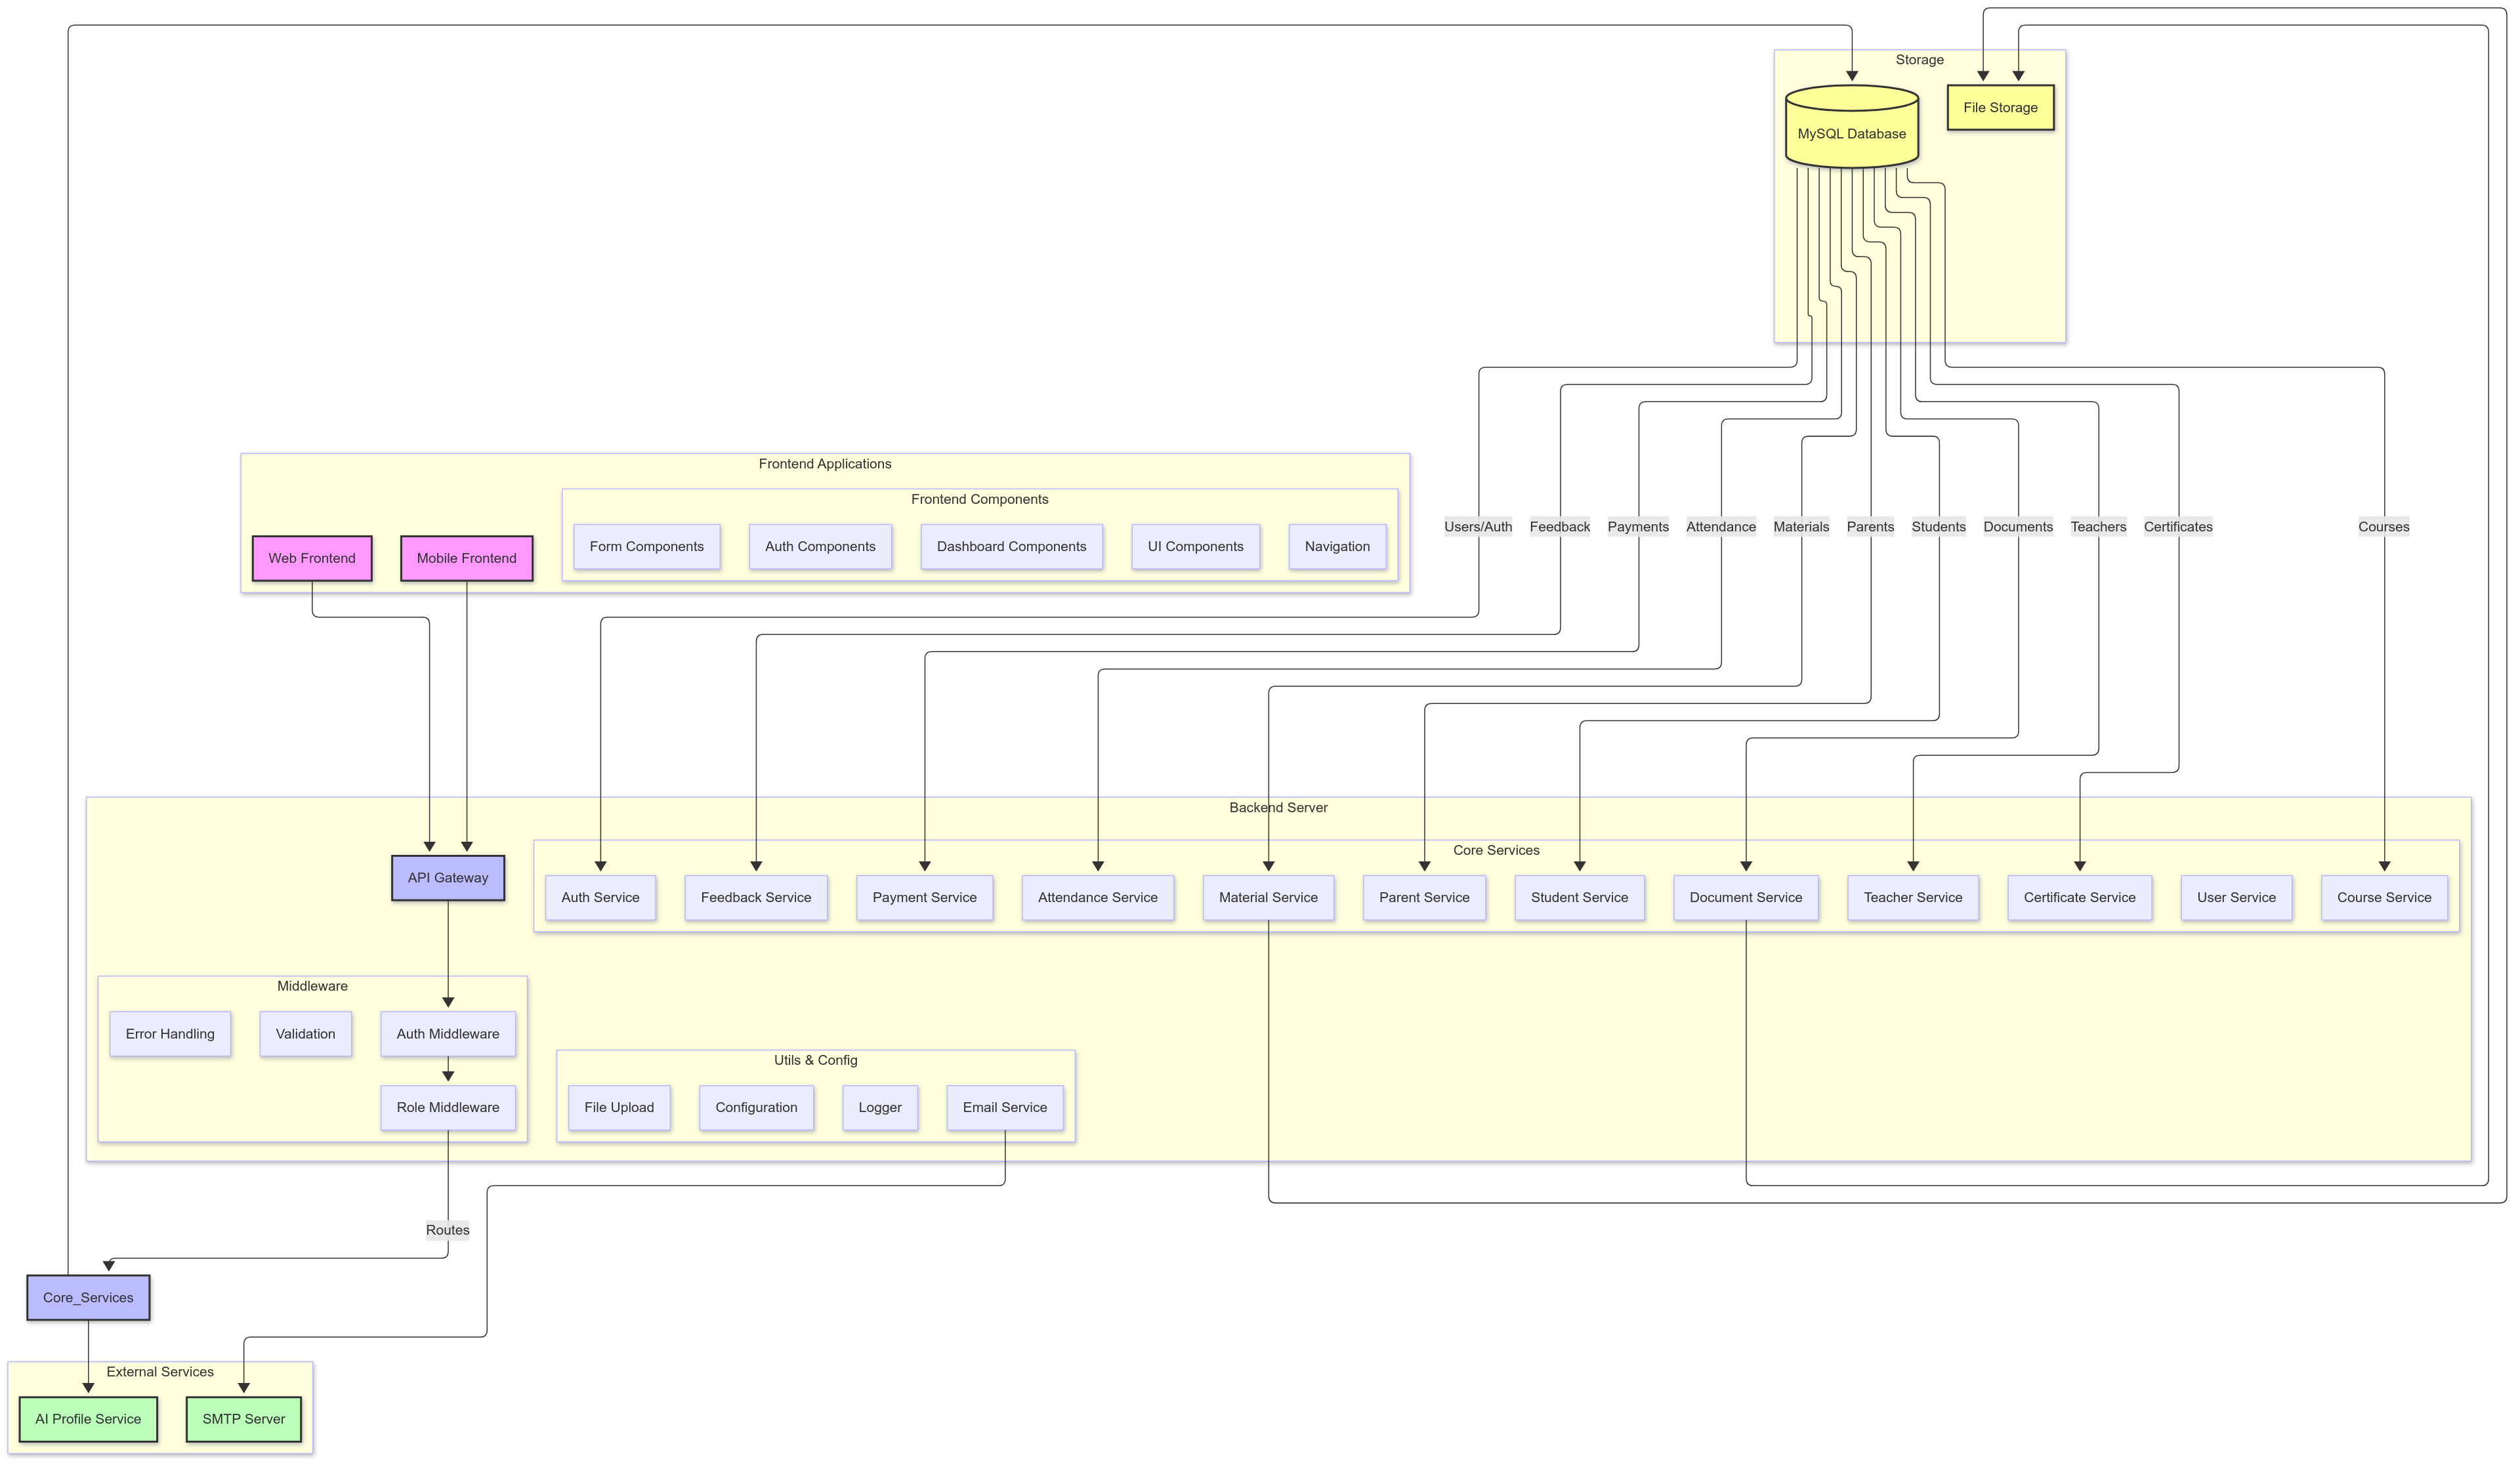
\includegraphics[width=0.9\textwidth,keepaspectratio]{pfe-pics/diagrames/archetecture.png}
  \caption{\textbf{Architecture globale} du système de gestion scolaire.}
  \label{fig:school_architecture}
\end{figure}

Cette architecture se compose de :

\begin{itemize}
  \item \textbf{Couche présentation} : Applications web et mobile offrant des interfaces adaptées à chaque type d'utilisateur
  
  \item \textbf{Couche API} : Services RESTful sécurisés exposant les fonctionnalités du système
  
  \item \textbf{Couche métier} : Implémentation de la logique métier et des règles de gestion
  
  \item \textbf{Couche persistance} : Gestion des données et interactions avec la base de données
  
  \item \textbf{Services transversaux} : Authentification, journalisation, gestion des fichiers, etc.
\end{itemize}

\subsection{Architecture du système de création de profils IA}

Le système de création de profils IA s'appuie sur une architecture orientée services, optimisée pour le traitement de documents et l'interaction avec des modèles d'IA :

\begin{itemize}
  \item \textbf{Frontend React/TypeScript} : Interface utilisateur réactive pour la gestion des profils et l'interaction avec l'IA
  
  \item \textbf{Backend FastAPI} : Services Python haute performance pour le traitement des documents et l'orchestration des modèles d'IA
  
  \item \textbf{Pipeline de traitement} : Système de traitement asynchrone pour l'extraction et l'analyse des contenus documentaires
  
  \item \textbf{Stockage hybride} : Combinaison de base de données PostgreSQL pour les métadonnées et de stockage objet pour les documents
  
  \item \textbf{Intégration IA} : Connecteurs vers des services d'IA externes (OpenRouter) pour le traitement du langage naturel
\end{itemize}

\section{Conception détaillée du système de gestion scolaire}

\subsection{Modèle de données}

Le modèle de données du système de gestion scolaire a été conçu pour représenter efficacement toutes les entités du domaine éducatif et leurs relations :

\begin{figure}[H]
  \centering
  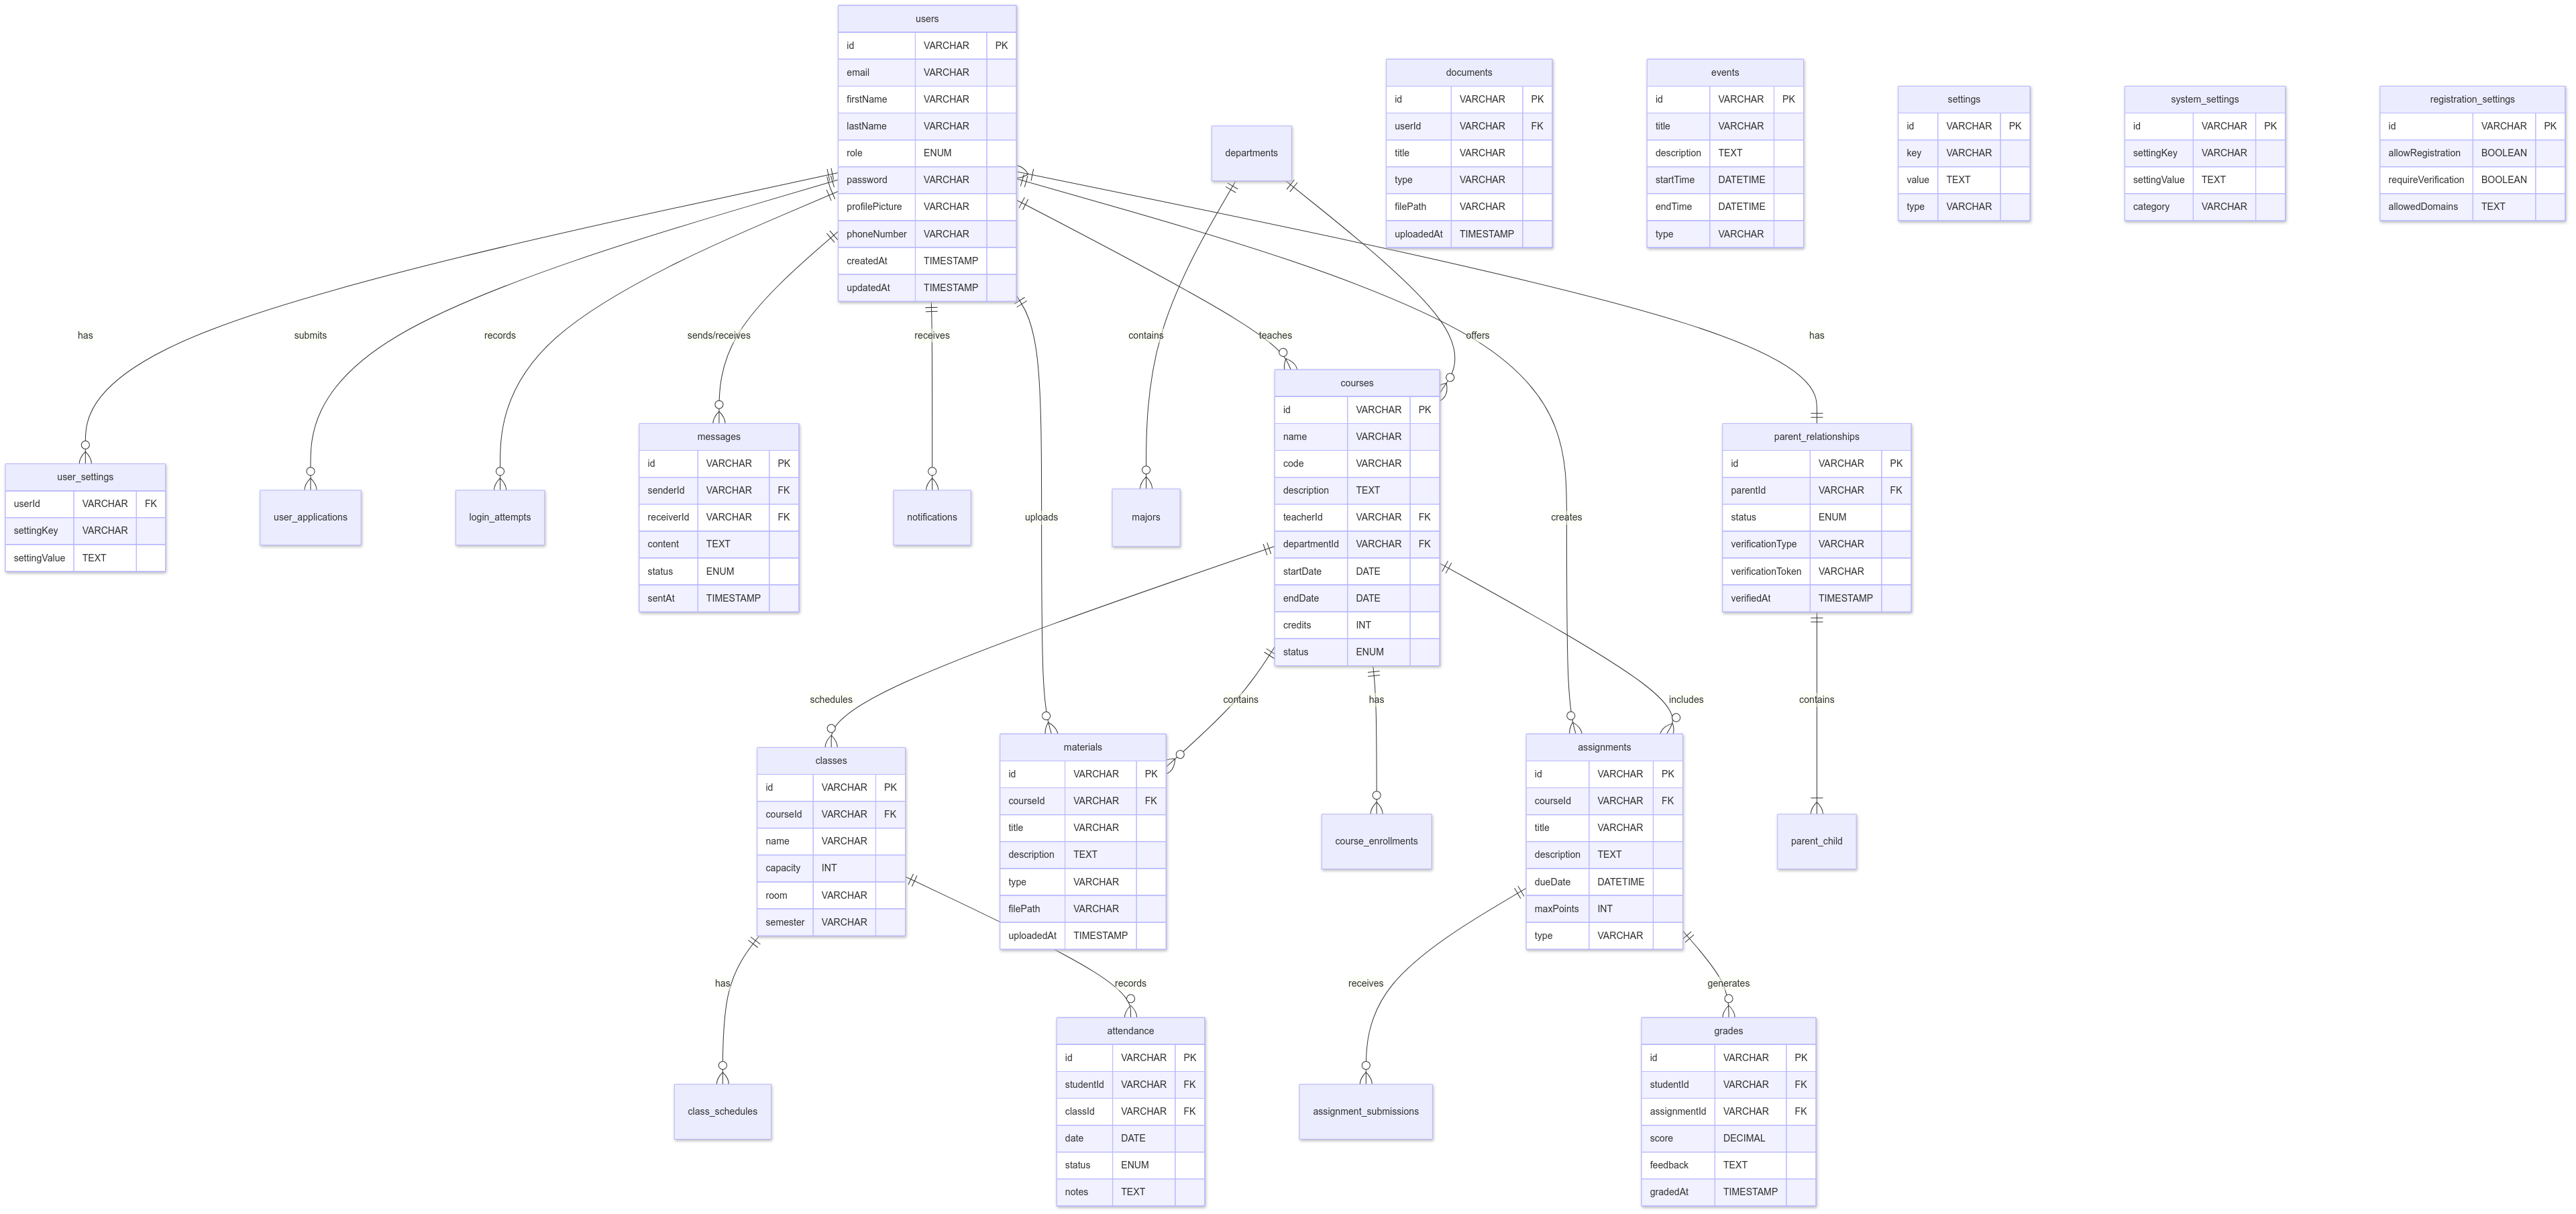
\includegraphics[width=0.9\textwidth,keepaspectratio]{pfe-pics/diagrames/tabaales.png}
  \caption{\textbf{Modèle de données} du système de gestion scolaire.}
  \label{fig:school_data_model}
\end{figure}

Les principales entités du modèle sont :

\begin{itemize}
  \item \textbf{User} : Entité de base pour tous les utilisateurs du système, avec spécialisation par rôle
  
  \item \textbf{Student} : Informations spécifiques aux étudiants, incluant leur parcours académique
  
  \item \textbf{Teacher} : Données relatives aux enseignants, incluant leurs spécialités et disponibilités
  
  \item \textbf{Parent} : Informations sur les parents et leurs relations avec les étudiants
  
  \item \textbf{Course} : Définition des cours avec leur contenu et organisation
  
  \item \textbf{Attendance} : Enregistrement des présences aux séances de cours
  
  \item \textbf{Assignment} : Travaux et évaluations assignés aux étudiants
  
  \item \textbf{Grade} : Notes et évaluations des étudiants
  
  \item \textbf{Notification} : Messages et alertes envoyés aux utilisateurs
  
  \item \textbf{Document} : Ressources pédagogiques et administratives partagées
\end{itemize}

\subsection{Diagramme de classes}

Le diagramme de classes détaille la structure objet du système et les relations entre les différentes classes :

\begin{figure}[H]
  \centering
  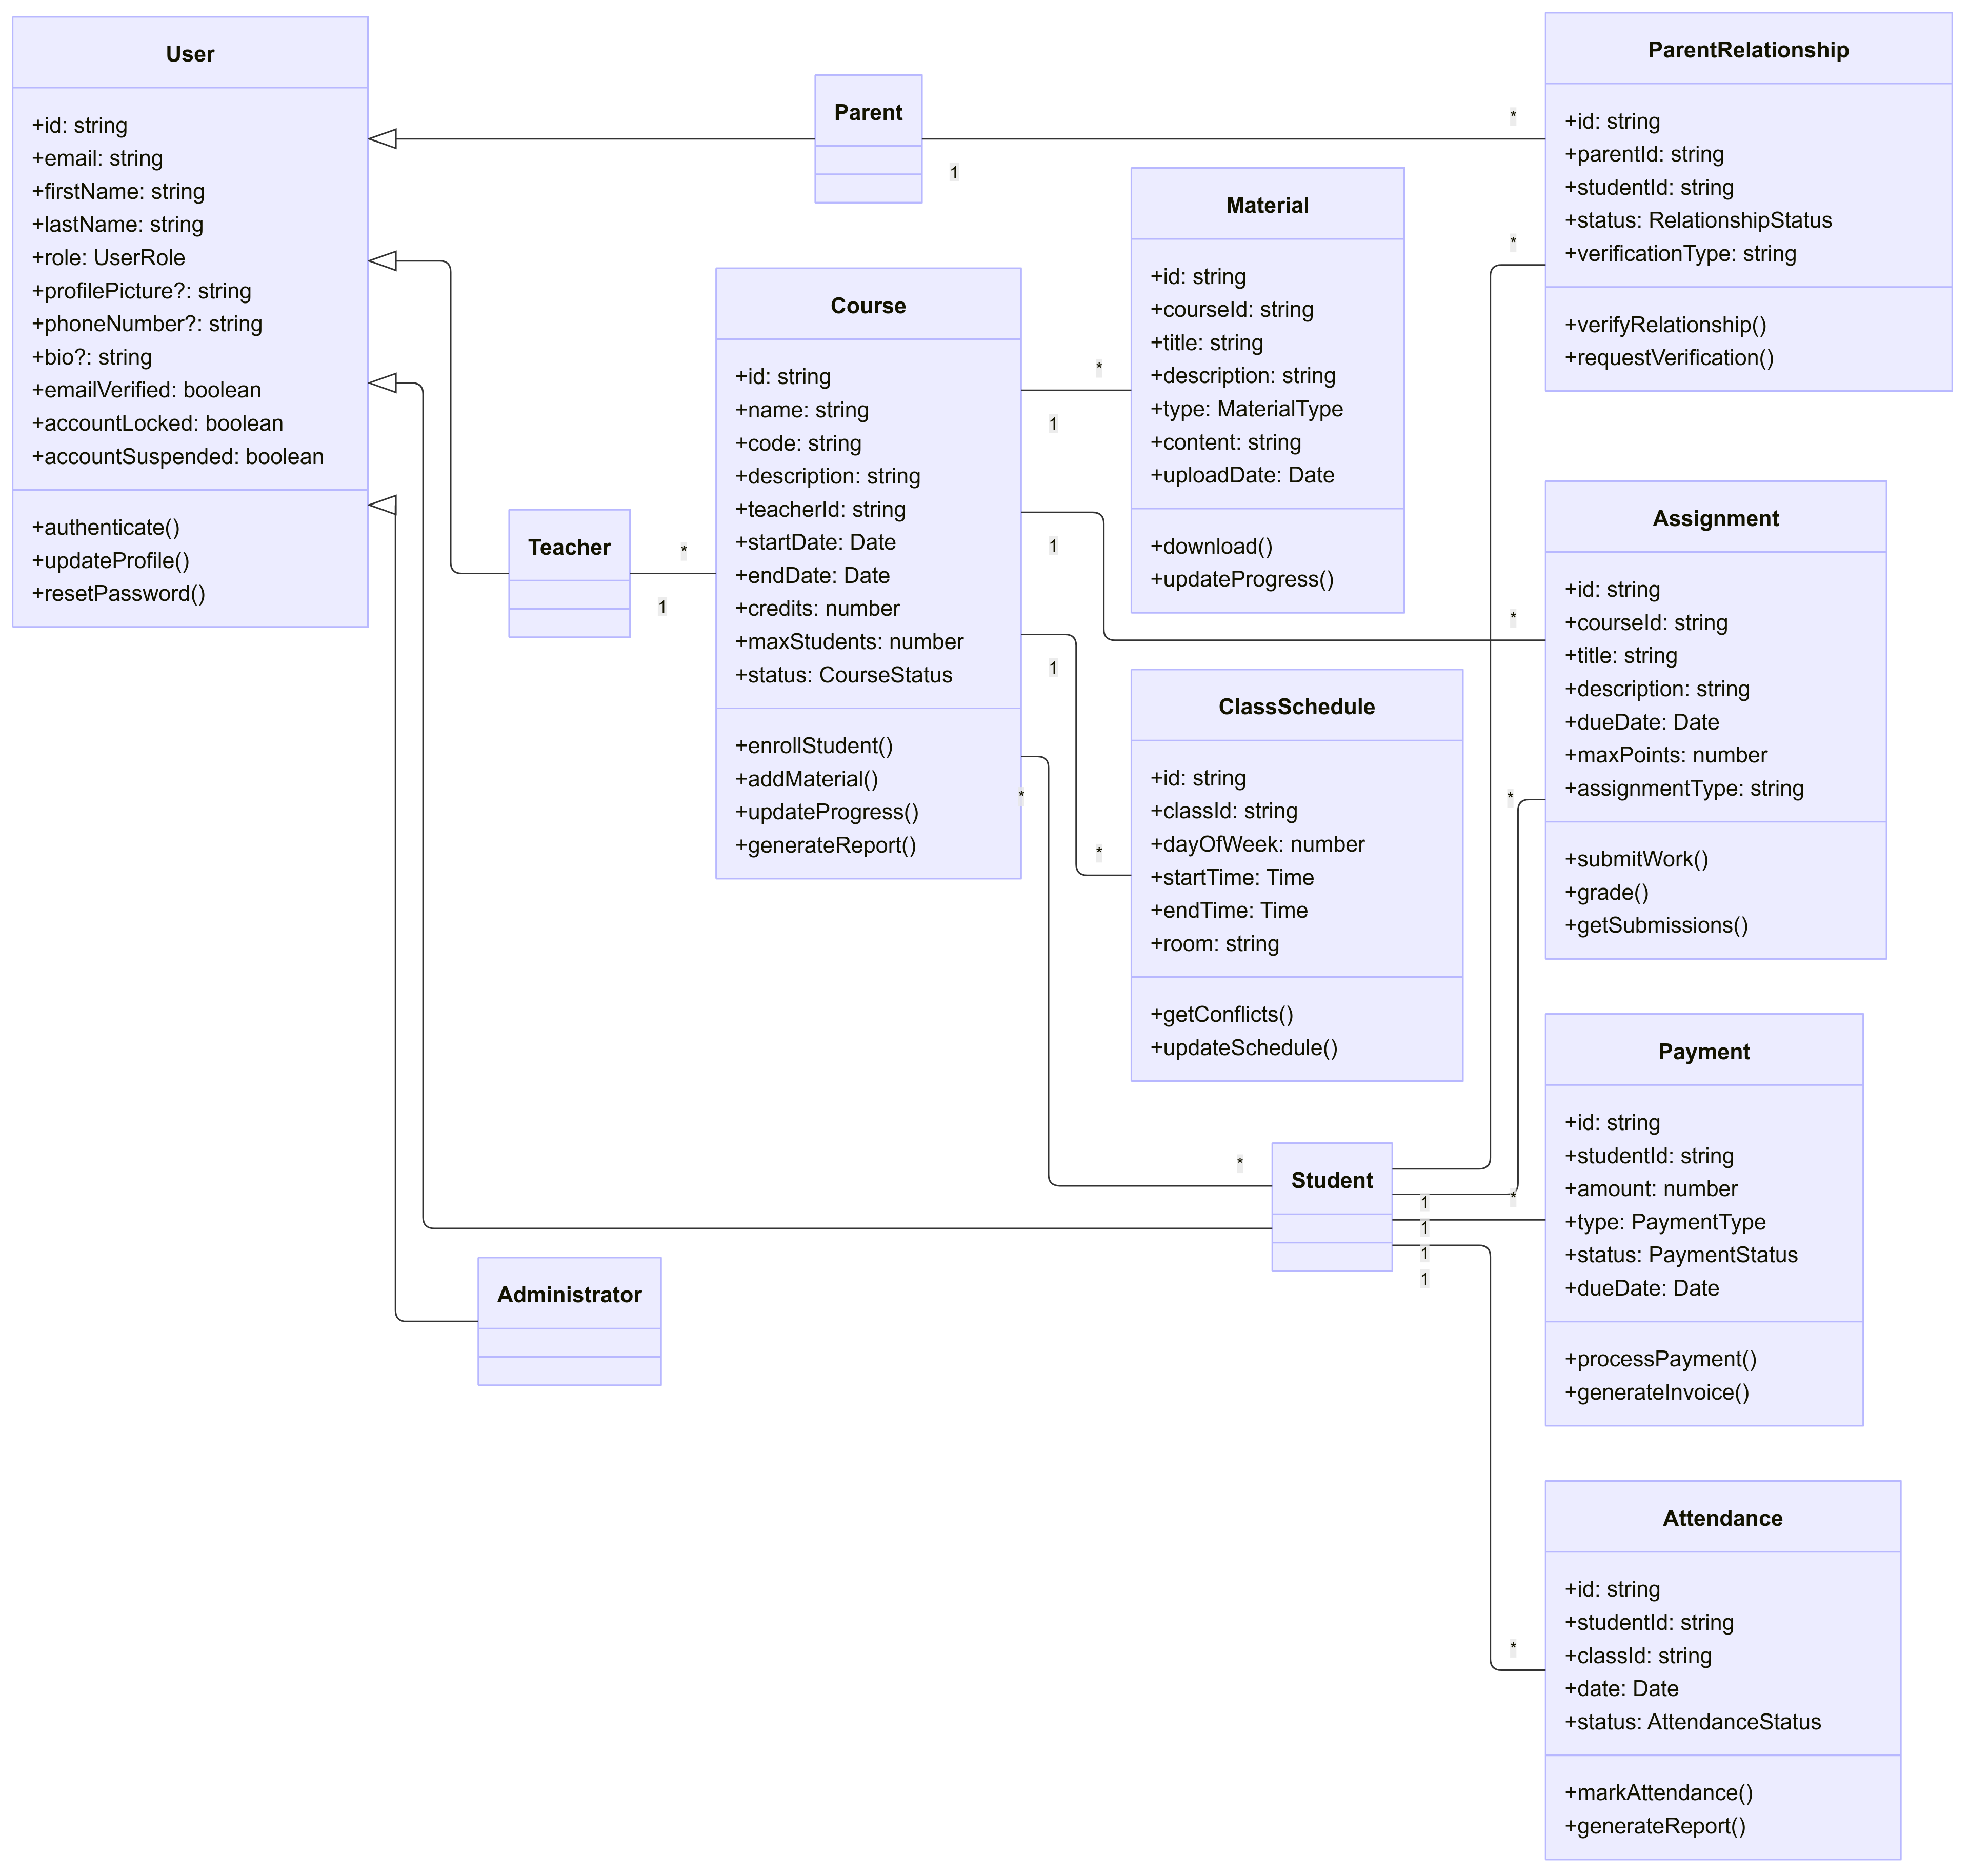
\includegraphics[width=0.9\textwidth,keepaspectratio]{pfe-pics/diagrames/class.png}
  \caption{\textbf{Diagramme de classes} du système de gestion scolaire.}
  \label{fig:school_class_diagram}
\end{figure}

Ce diagramme met en évidence :

\begin{itemize}
  \item Les attributs et méthodes clés de chaque classe
  
  \item Les relations d'héritage, notamment pour les différents types d'utilisateurs
  
  \item Les associations entre classes, avec leur cardinalité
  
  \item Les agrégations et compositions représentant les relations de contenance
\end{itemize}

\subsection{Architecture frontend}

L'architecture frontend du système de gestion scolaire repose sur une approche modulaire et réactive :

\subsubsection{Application web}

L'application web utilise React avec TypeScript et adopte une architecture basée sur les composants :

\begin{itemize}
  \item \textbf{Structure des composants} : Organisation hiérarchique avec composants atomiques, moléculaires et organismes
  
  \item \textbf{Gestion d'état} : Utilisation de Context API et hooks personnalisés pour la gestion de l'état global
  
  \item \textbf{Routage} : Système de navigation basé sur React Router avec gestion des autorisations
  
  \item \textbf{Thème et styles} : Approche basée sur Tailwind CSS avec thèmes personnalisables
  
  \item \textbf{Internationalisation} : Support multilingue avec gestion des traductions
\end{itemize}

\subsubsection{Application mobile}

L'application mobile est développée avec React Native, partageant une partie de la logique avec l'application web :

\begin{itemize}
  \item \textbf{Navigation native} : Utilisation de React Navigation pour une expérience fluide
  
  \item \textbf{Composants adaptatifs} : Interface optimisée pour les interactions tactiles
  
  \item \textbf{Fonctionnalités natives} : Intégration des notifications push, de l'appareil photo et du stockage local
  
  \item \textbf{Mode hors ligne} : Synchronisation des données pour utilisation sans connexion permanente
\end{itemize}

\subsection{Architecture backend}

Le backend du système de gestion scolaire est conçu selon une architecture en couches avec une séparation claire des responsabilités :

\begin{itemize}
  \item \textbf{Couche API} : Contrôleurs REST exposant les endpoints du système
  
  \item \textbf{Couche service} : Implémentation de la logique métier et orchestration des opérations
  
  \item \textbf{Couche repository} : Abstraction des opérations de persistance et requêtes à la base de données
  
  \item \textbf{Couche entité} : Modèles de données et mappings ORM
  
  \item \textbf{Services transversaux} : Authentification, autorisation, validation, journalisation
\end{itemize}

\subsection{Flux de travail principaux}

Plusieurs flux de travail clés ont été modélisés pour guider l'implémentation :

\subsubsection{Processus d'authentification}

\begin{figure}[H]
  \centering
  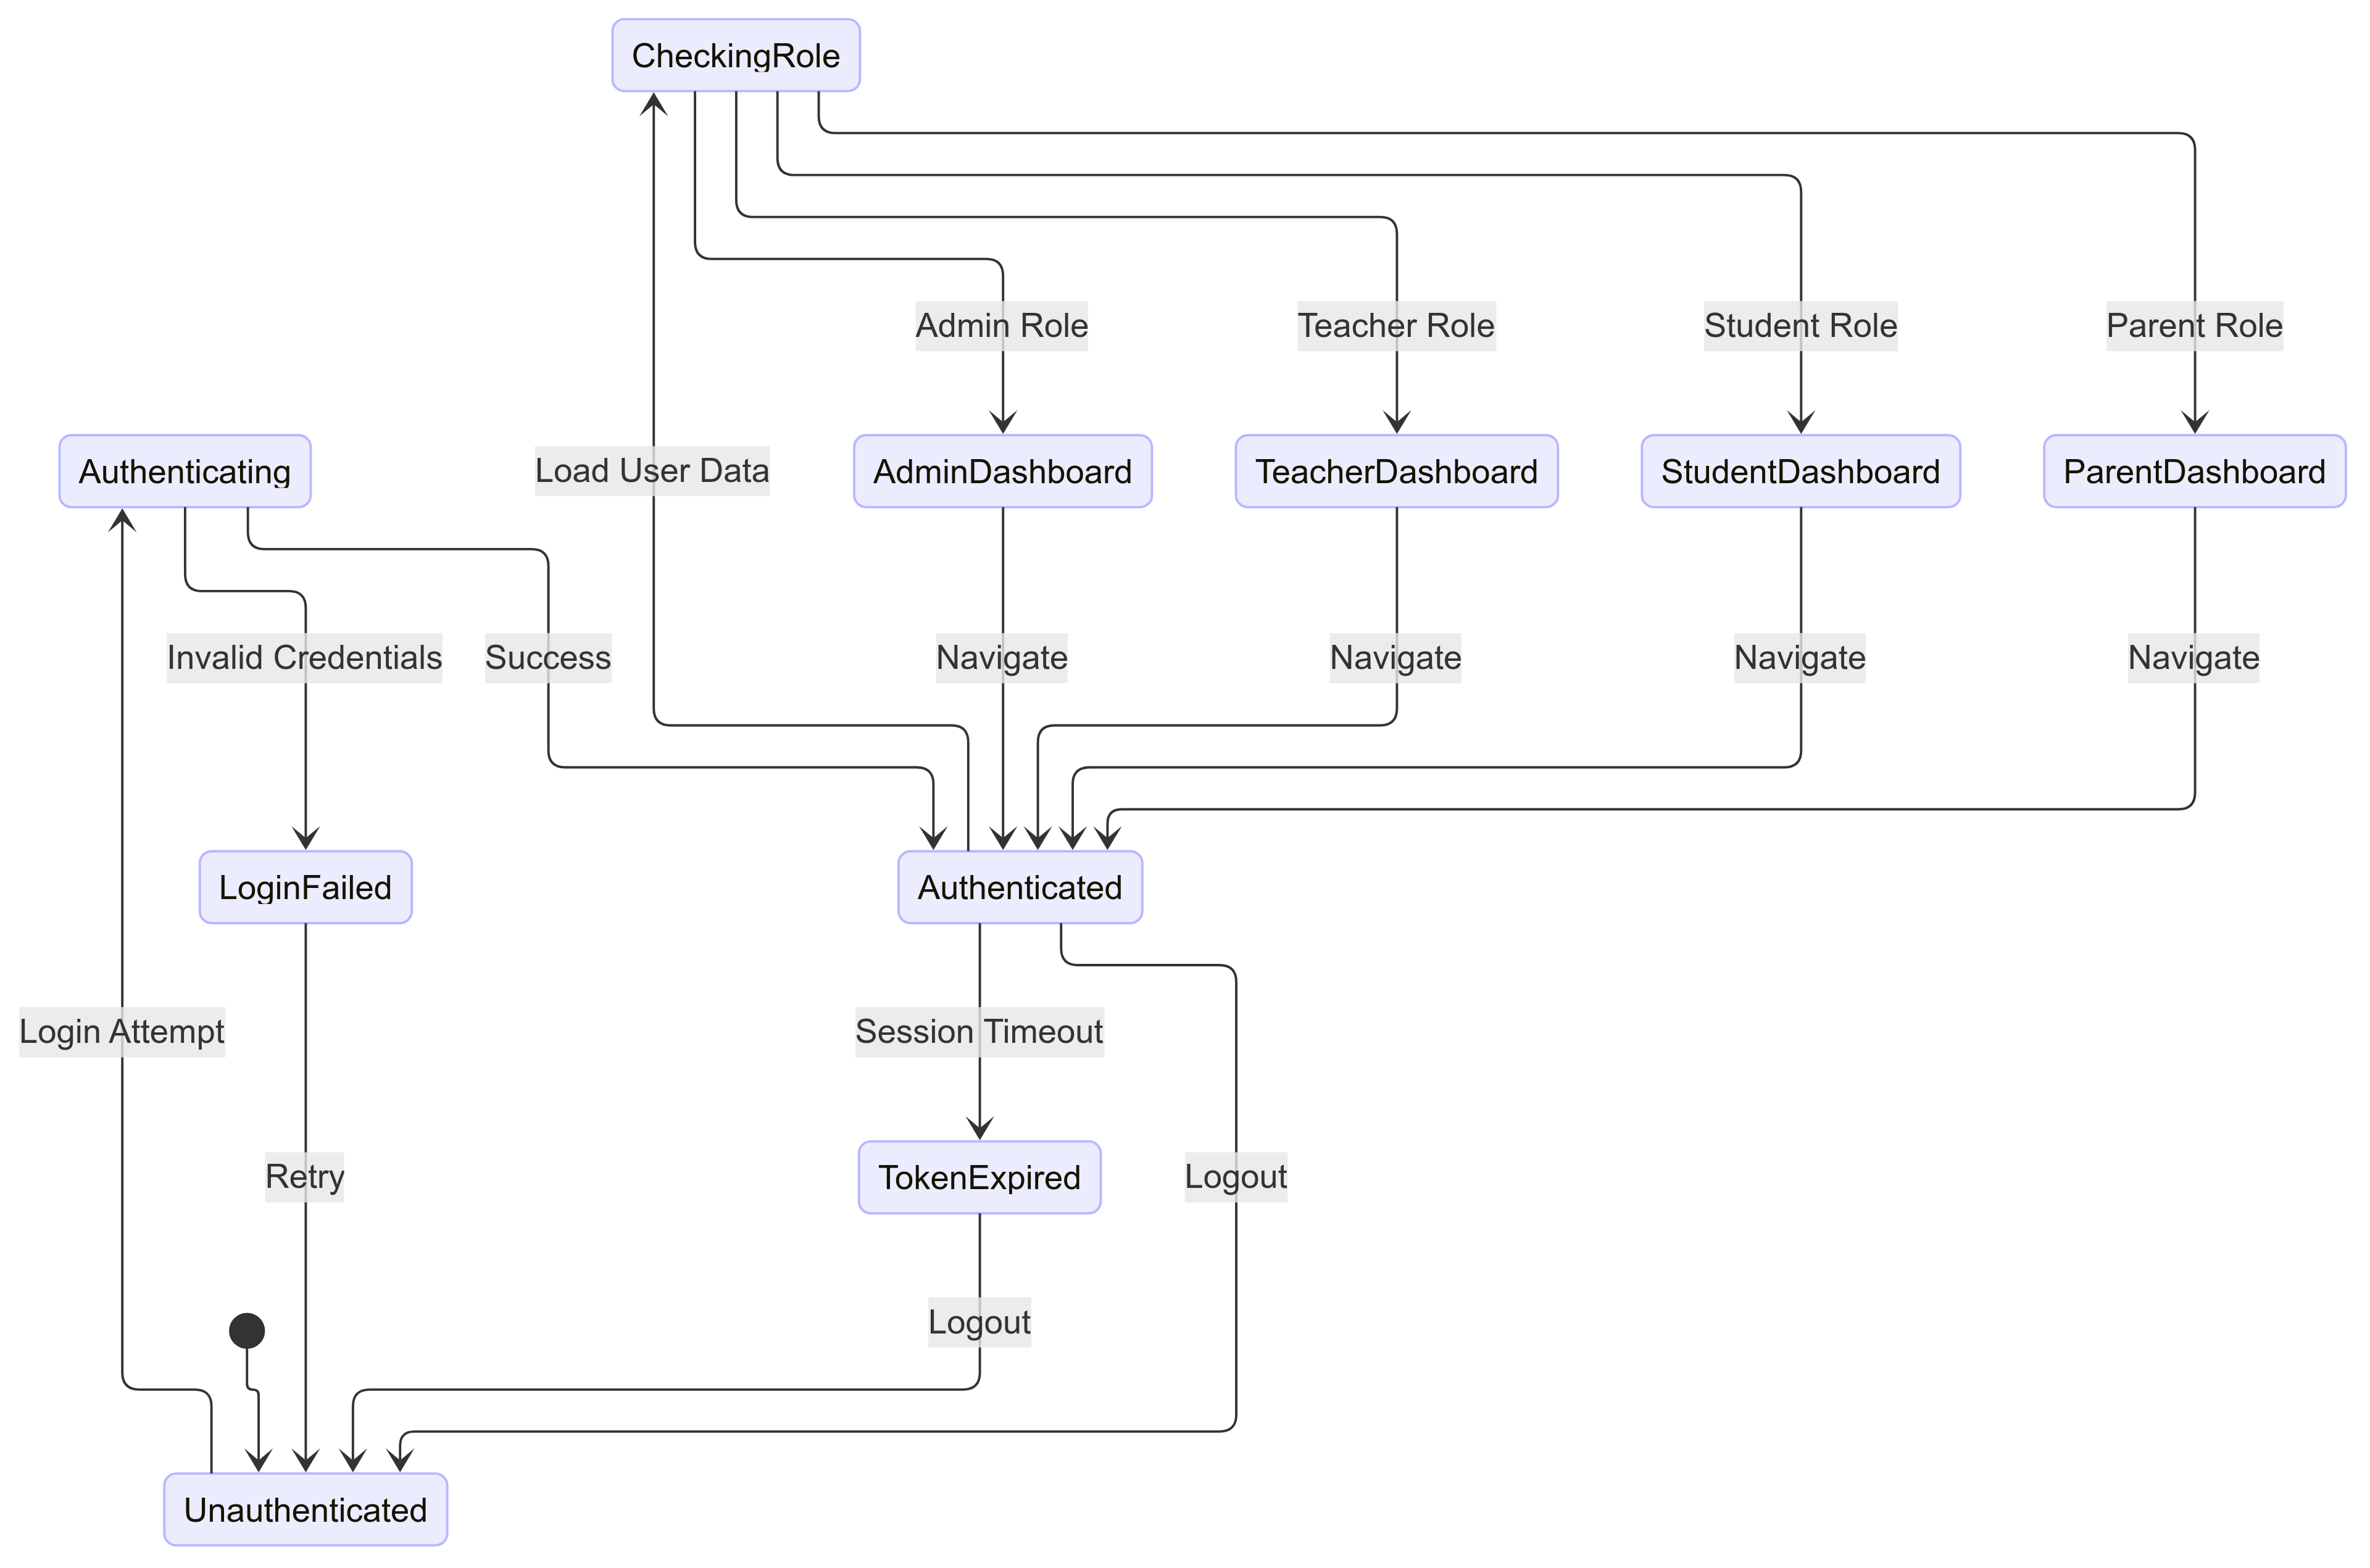
\includegraphics[width=0.9\textwidth,keepaspectratio]{pfe-pics/diagrames/State Diagram (for Authentication Flow).png}
  \caption{\textbf{Diagramme d'états} pour le processus d'authentification.}
  \label{fig:auth_flow}
\end{figure}

Ce diagramme illustre :

\begin{itemize}
  \item Les différents états possibles du processus d'authentification
  
  \item Les transitions entre ces états en fonction des actions utilisateur
  
  \item Les vérifications de sécurité à chaque étape
  
  \item La gestion des erreurs et des cas particuliers
\end{itemize}

\subsubsection{Gestion des cours}

\begin{figure}[H]
  \centering
  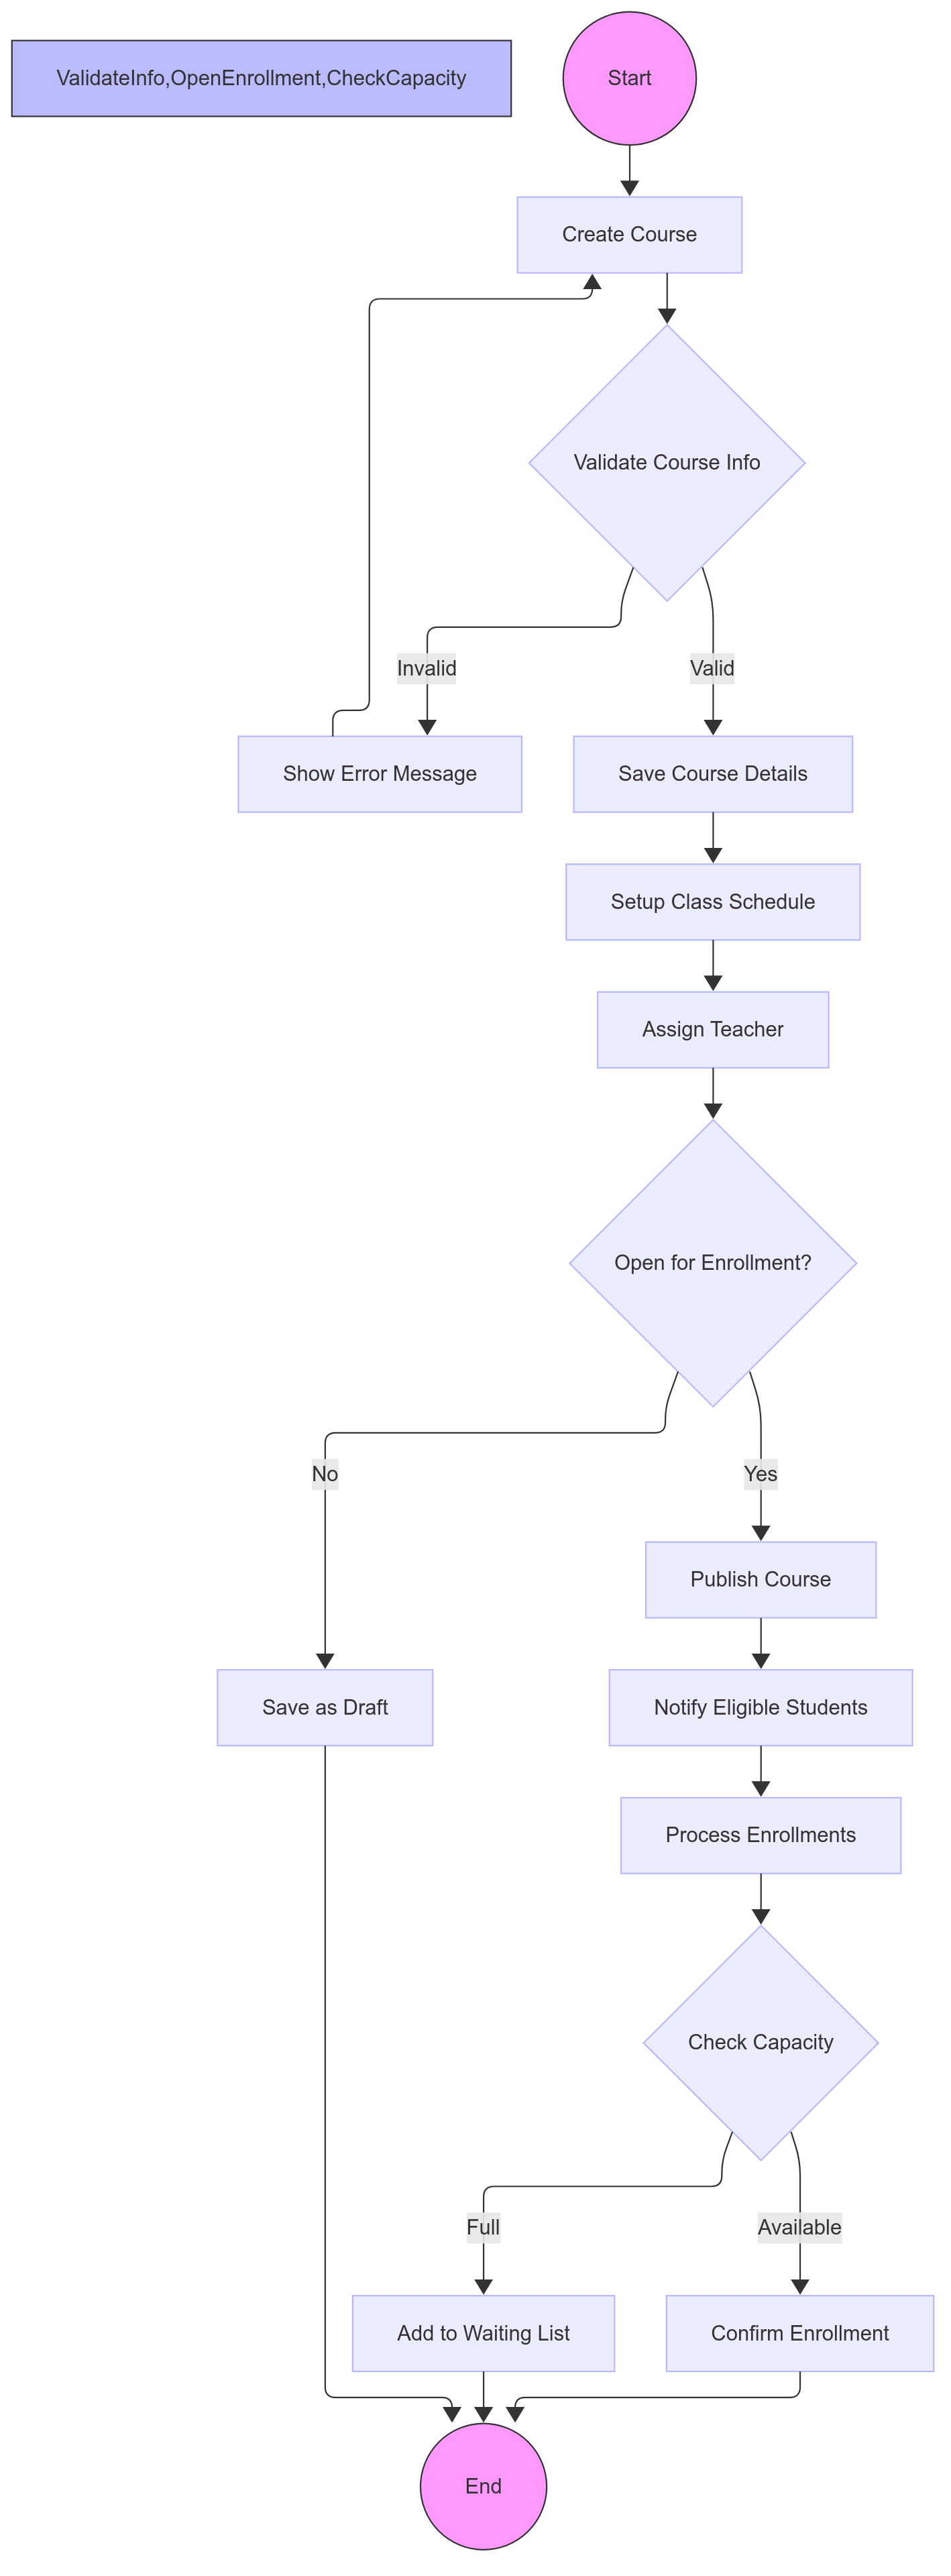
\includegraphics[width=0.9\textwidth,keepaspectratio]{pfe-pics/diagrames/Activity Diagram (for Course Management).png}
  \caption{\textbf{Diagramme d'activité} pour la gestion des cours.}
  \label{fig:course_management}
\end{figure}

Ce flux détaille :

\begin{itemize}
  \item Les étapes de création et configuration d'un cours
  
  \item L'assignation des enseignants et l'inscription des étudiants
  
  \item La gestion du matériel pédagogique
  
  \item Le suivi et l'évaluation des activités du cours
\end{itemize}

\subsubsection{Suivi des présences}

\begin{figure}[H]
  \centering
  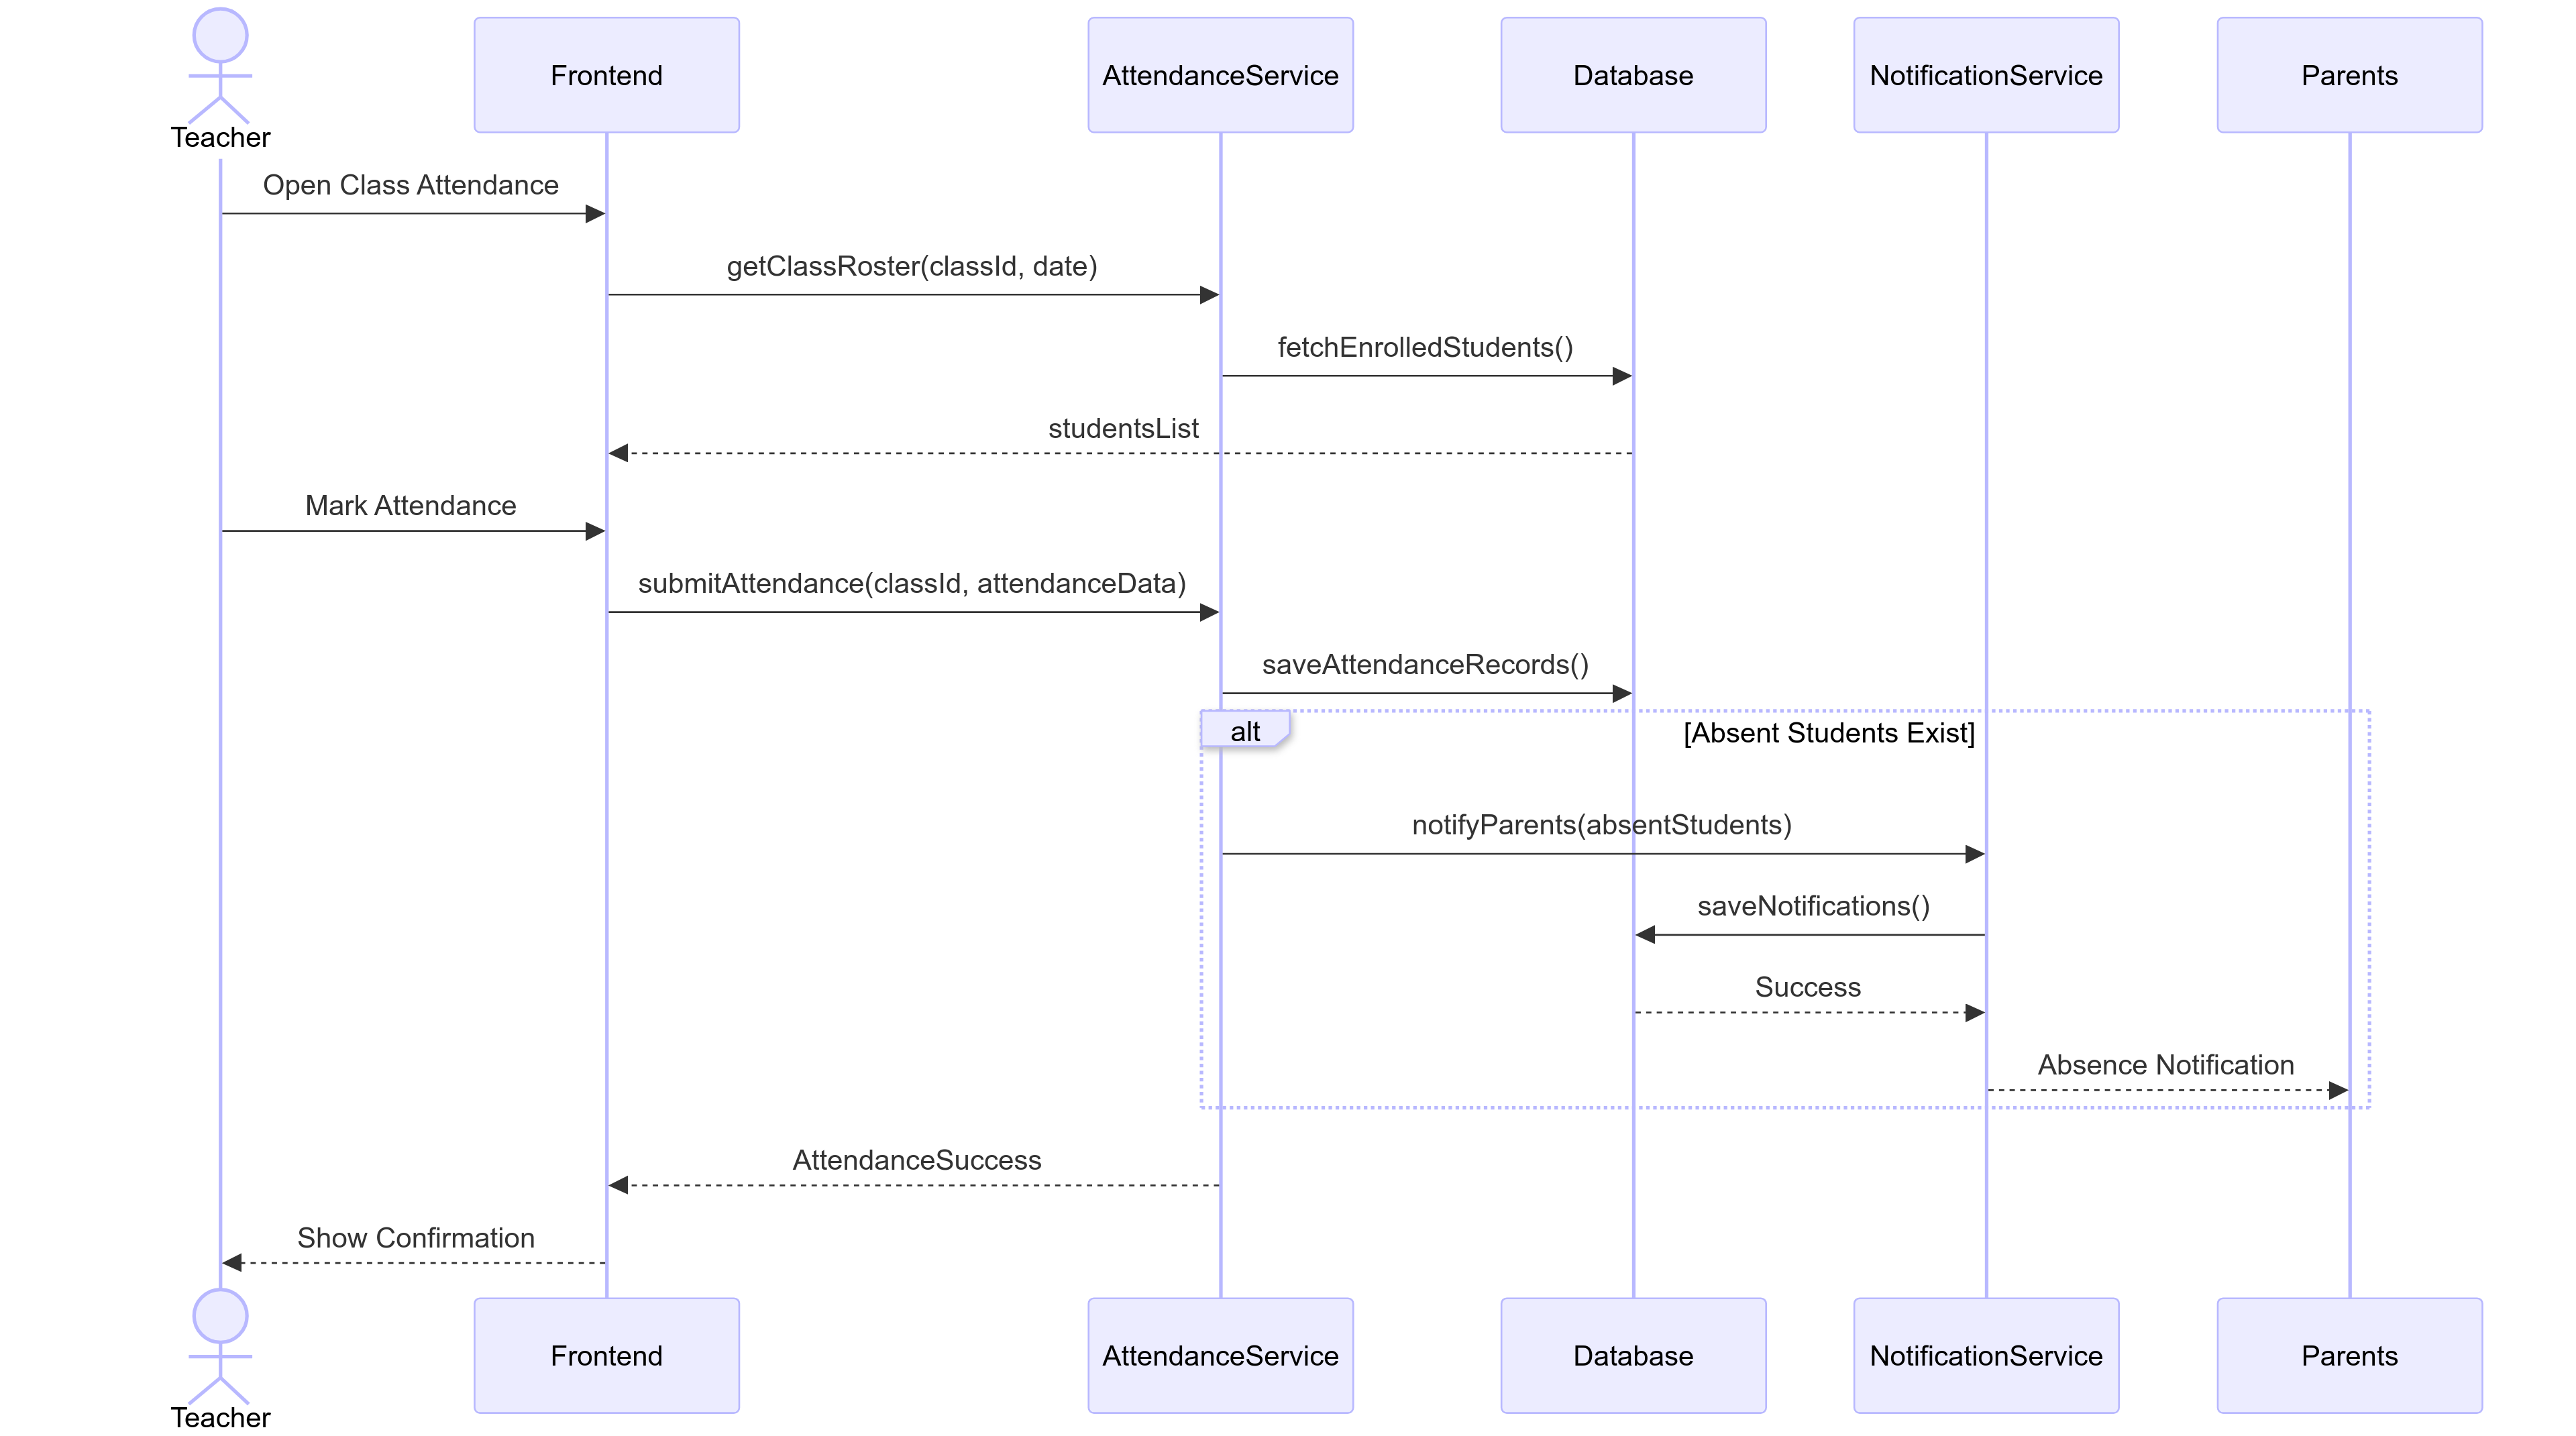
\includegraphics[width=0.9\textwidth,keepaspectratio]{pfe-pics/diagrames/Attendance Tracking.png}
  \caption{\textbf{Diagramme de séquence} pour le suivi des présences.}
  \label{fig:attendance_tracking}
\end{figure}

Ce diagramme montre :

\begin{itemize}
  \item Les interactions entre l'enseignant et le système pour l'enregistrement des présences
  
  \item La validation et la persistance des données d'assiduité
  
  \item Les notifications automatiques en cas d'absence
  
  \item La consultation des rapports de présence par les différents acteurs
\end{itemize}

\subsubsection{Soumission et notation des devoirs}

\begin{figure}[H]
  \centering
  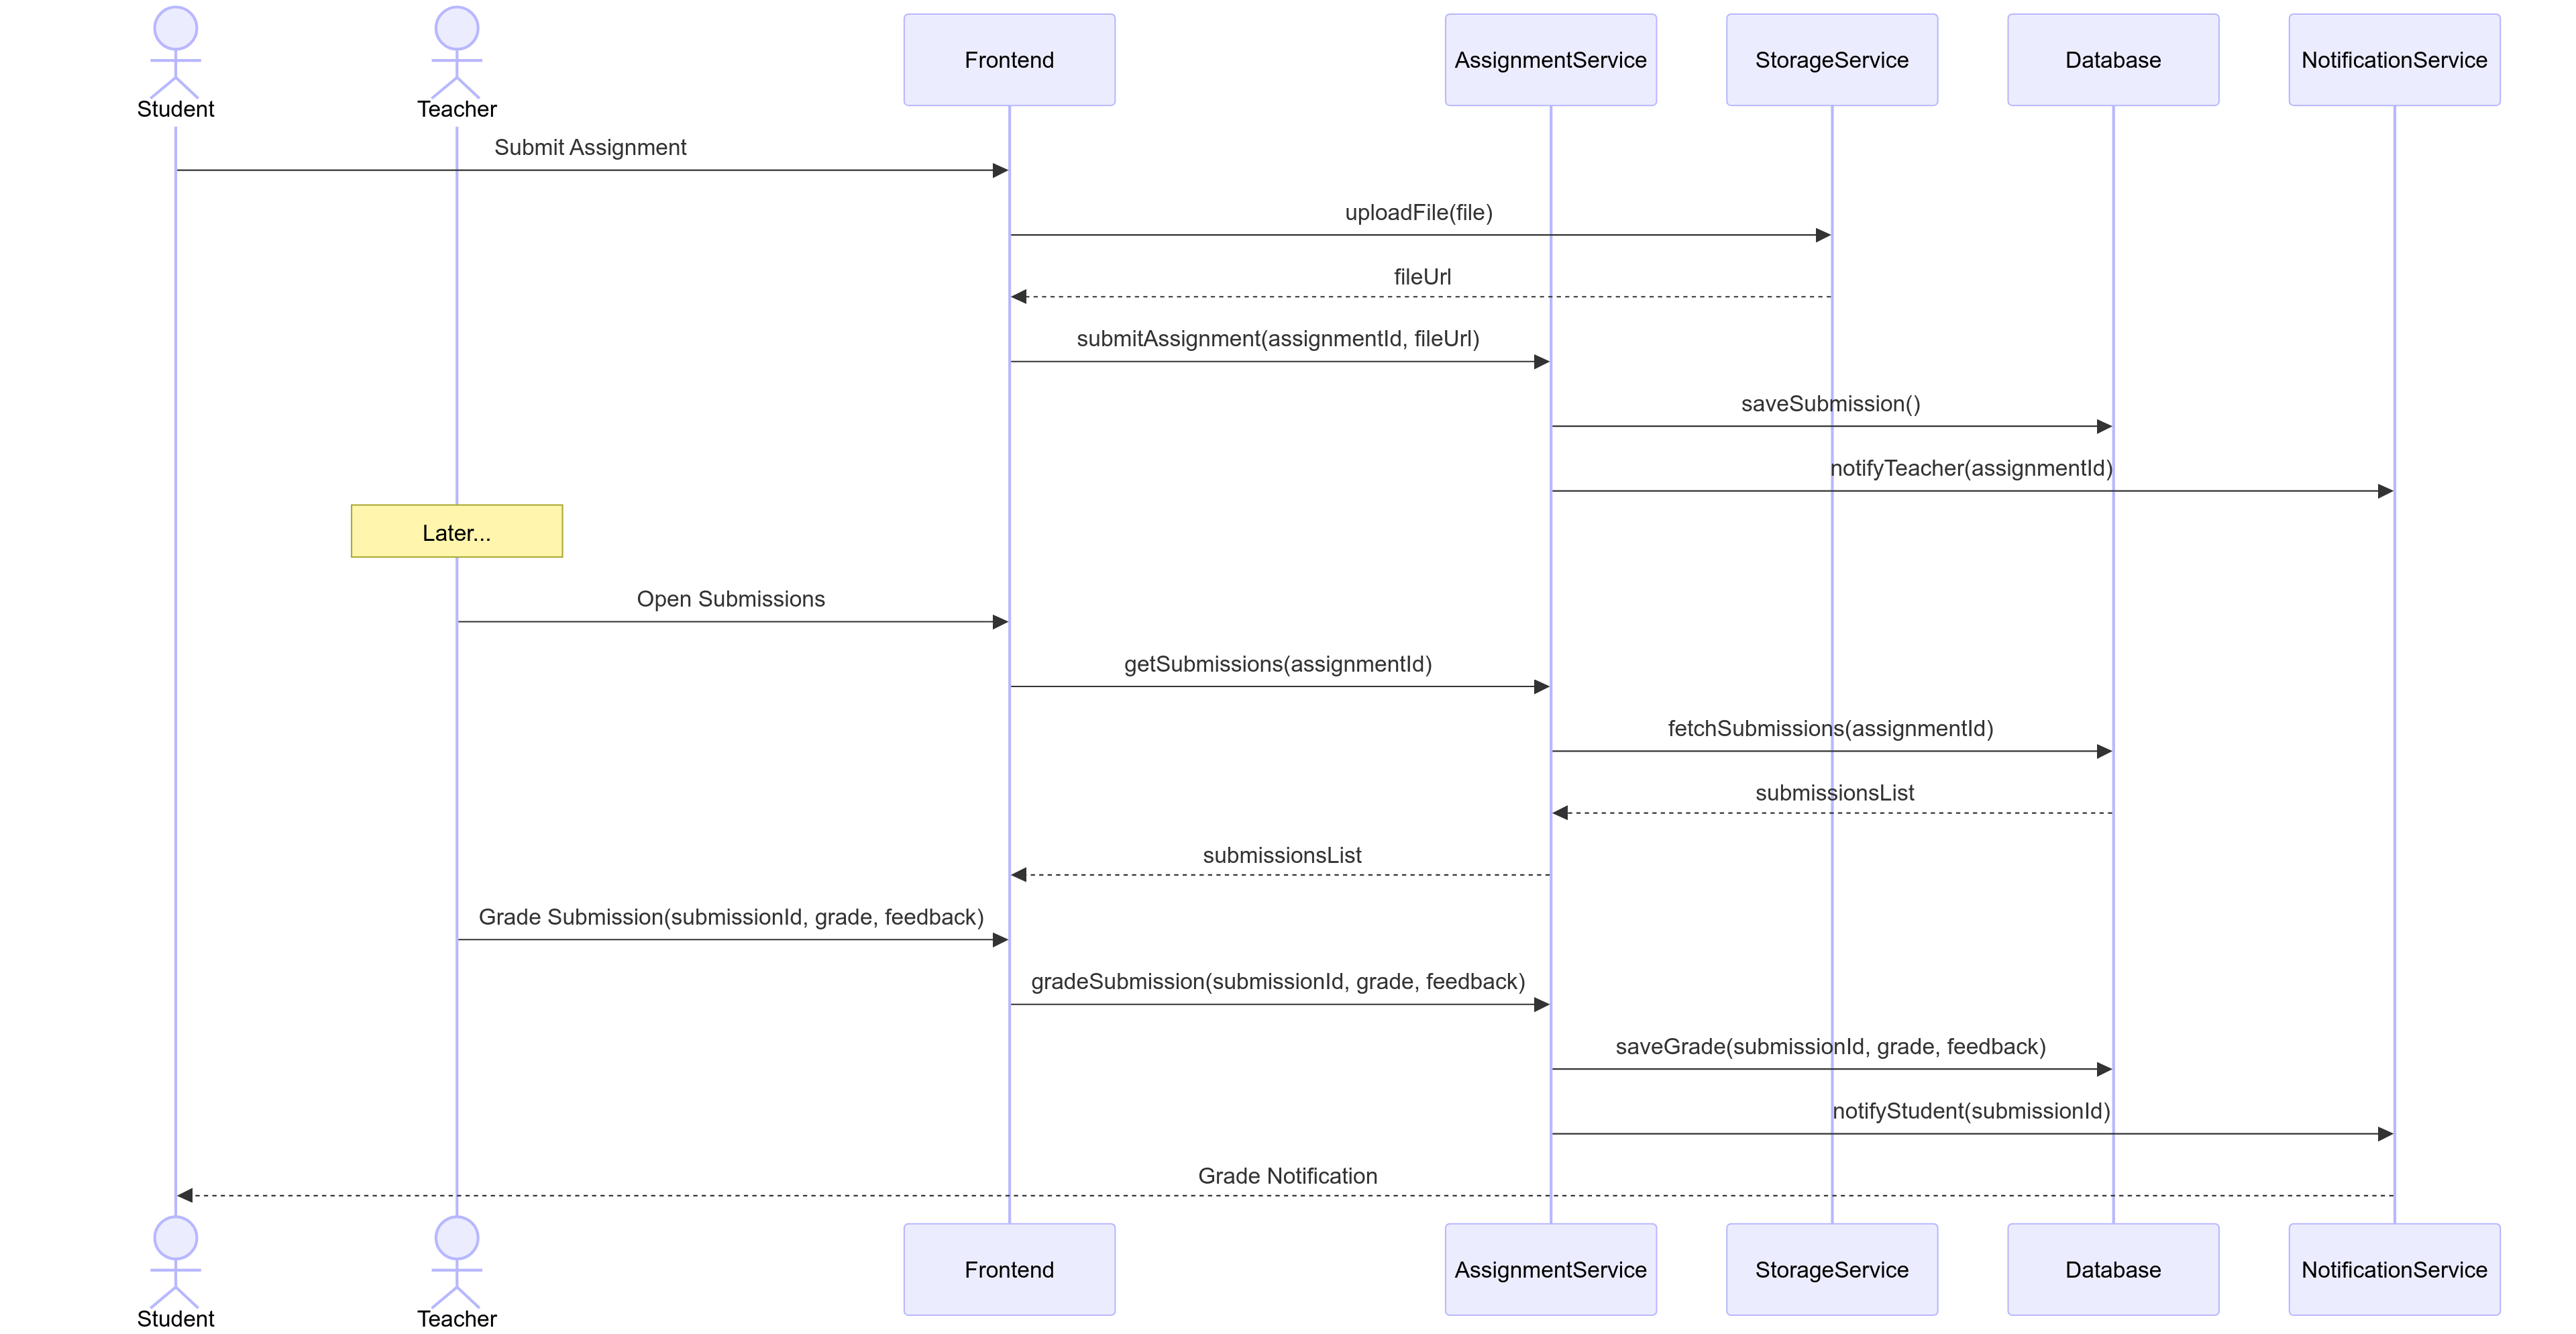
\includegraphics[width=0.9\textwidth,keepaspectratio]{pfe-pics/diagrames/Assignment Submission and Grading.png}
  \caption{\textbf{Diagramme de flux} pour la soumission et notation des devoirs.}
  \label{fig:assignment_grading}
\end{figure}

Ce flux illustre :

\begin{itemize}
  \item La création et l'assignation de travaux par l'enseignant
  
  \item La soumission des travaux par les étudiants
  
  \item Le processus d'évaluation et de feedback
  
  \item La publication et consultation des résultats
\end{itemize}

\subsubsection{Vérification parent-enfant}

\begin{figure}[H]
  \centering
  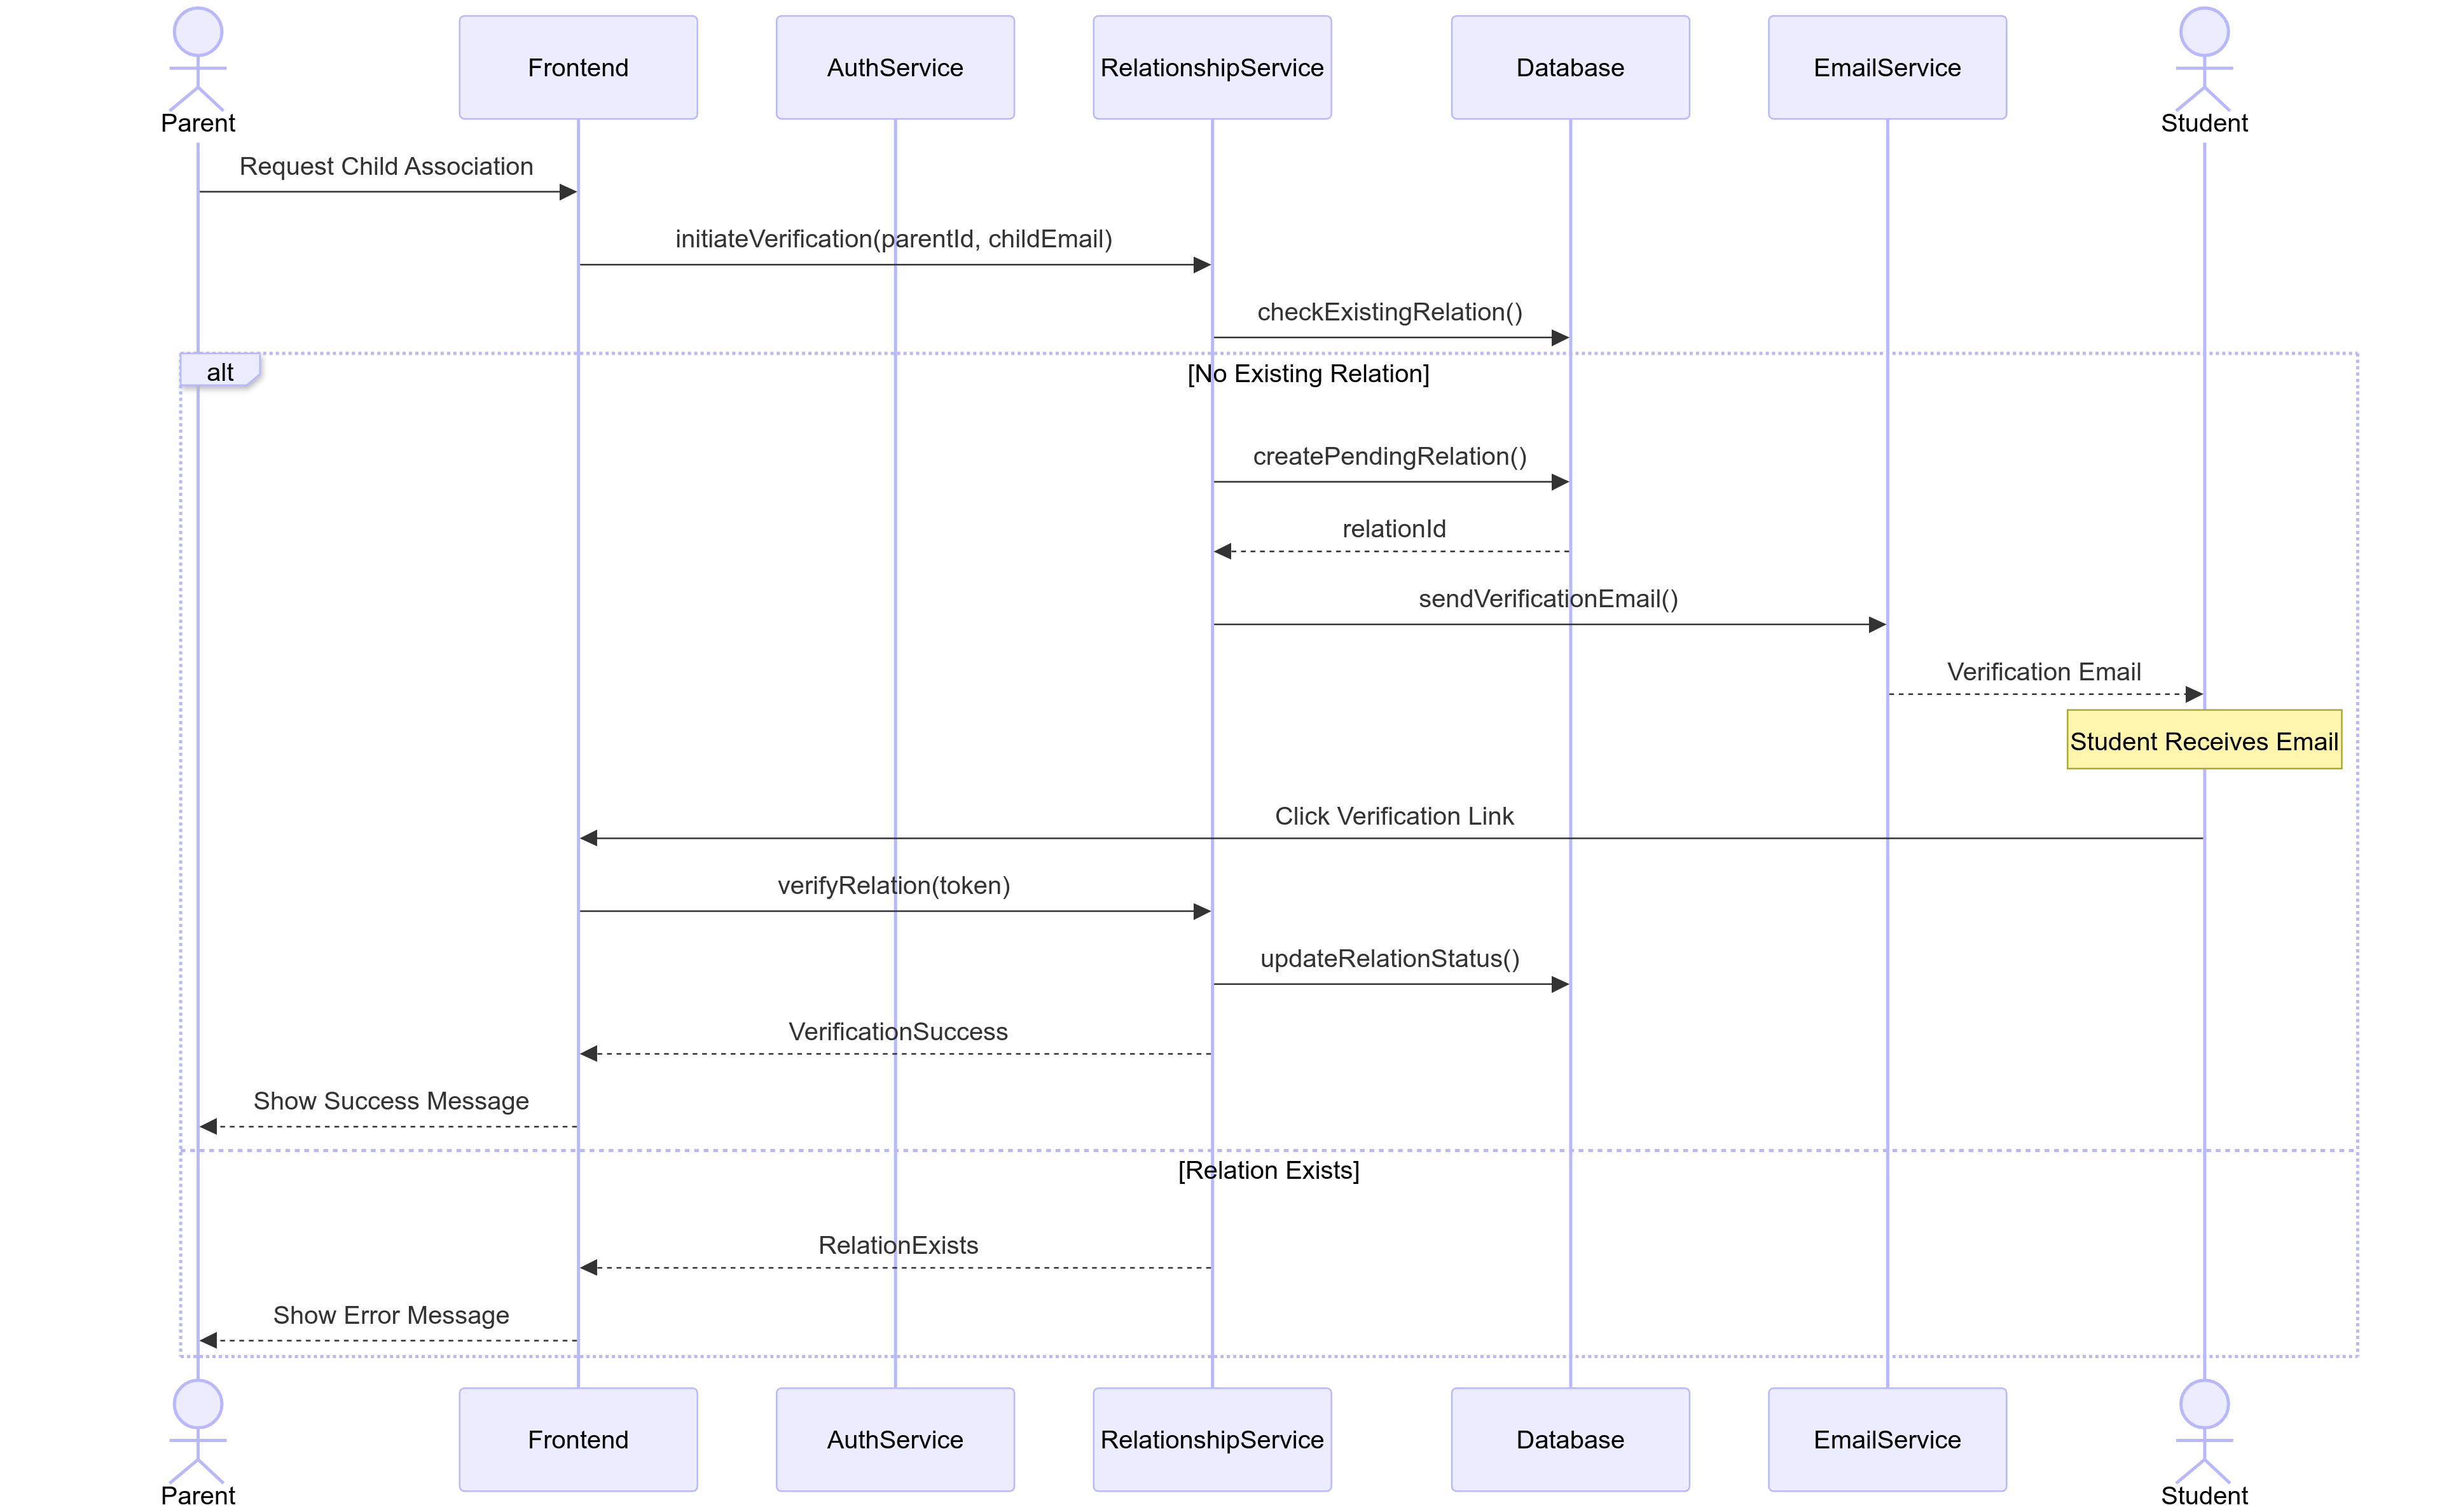
\includegraphics[width=0.9\textwidth,keepaspectratio]{pfe-pics/diagrames/Parent-Child Verification Process.png}
  \caption{\textbf{Diagramme de processus} pour la vérification parent-enfant.}
  \label{fig:parent_child_verification}
\end{figure}

Ce processus sécurisé détaille :

\begin{itemize}
  \item L'initiation de la demande d'association par le parent
  
  \item La vérification des informations fournies
  
  \item La validation par l'administration
  
  \item L'établissement de la relation parent-enfant dans le système
\end{itemize}

\subsubsection{Inscription aux cours}

\begin{figure}[H]
  \centering
  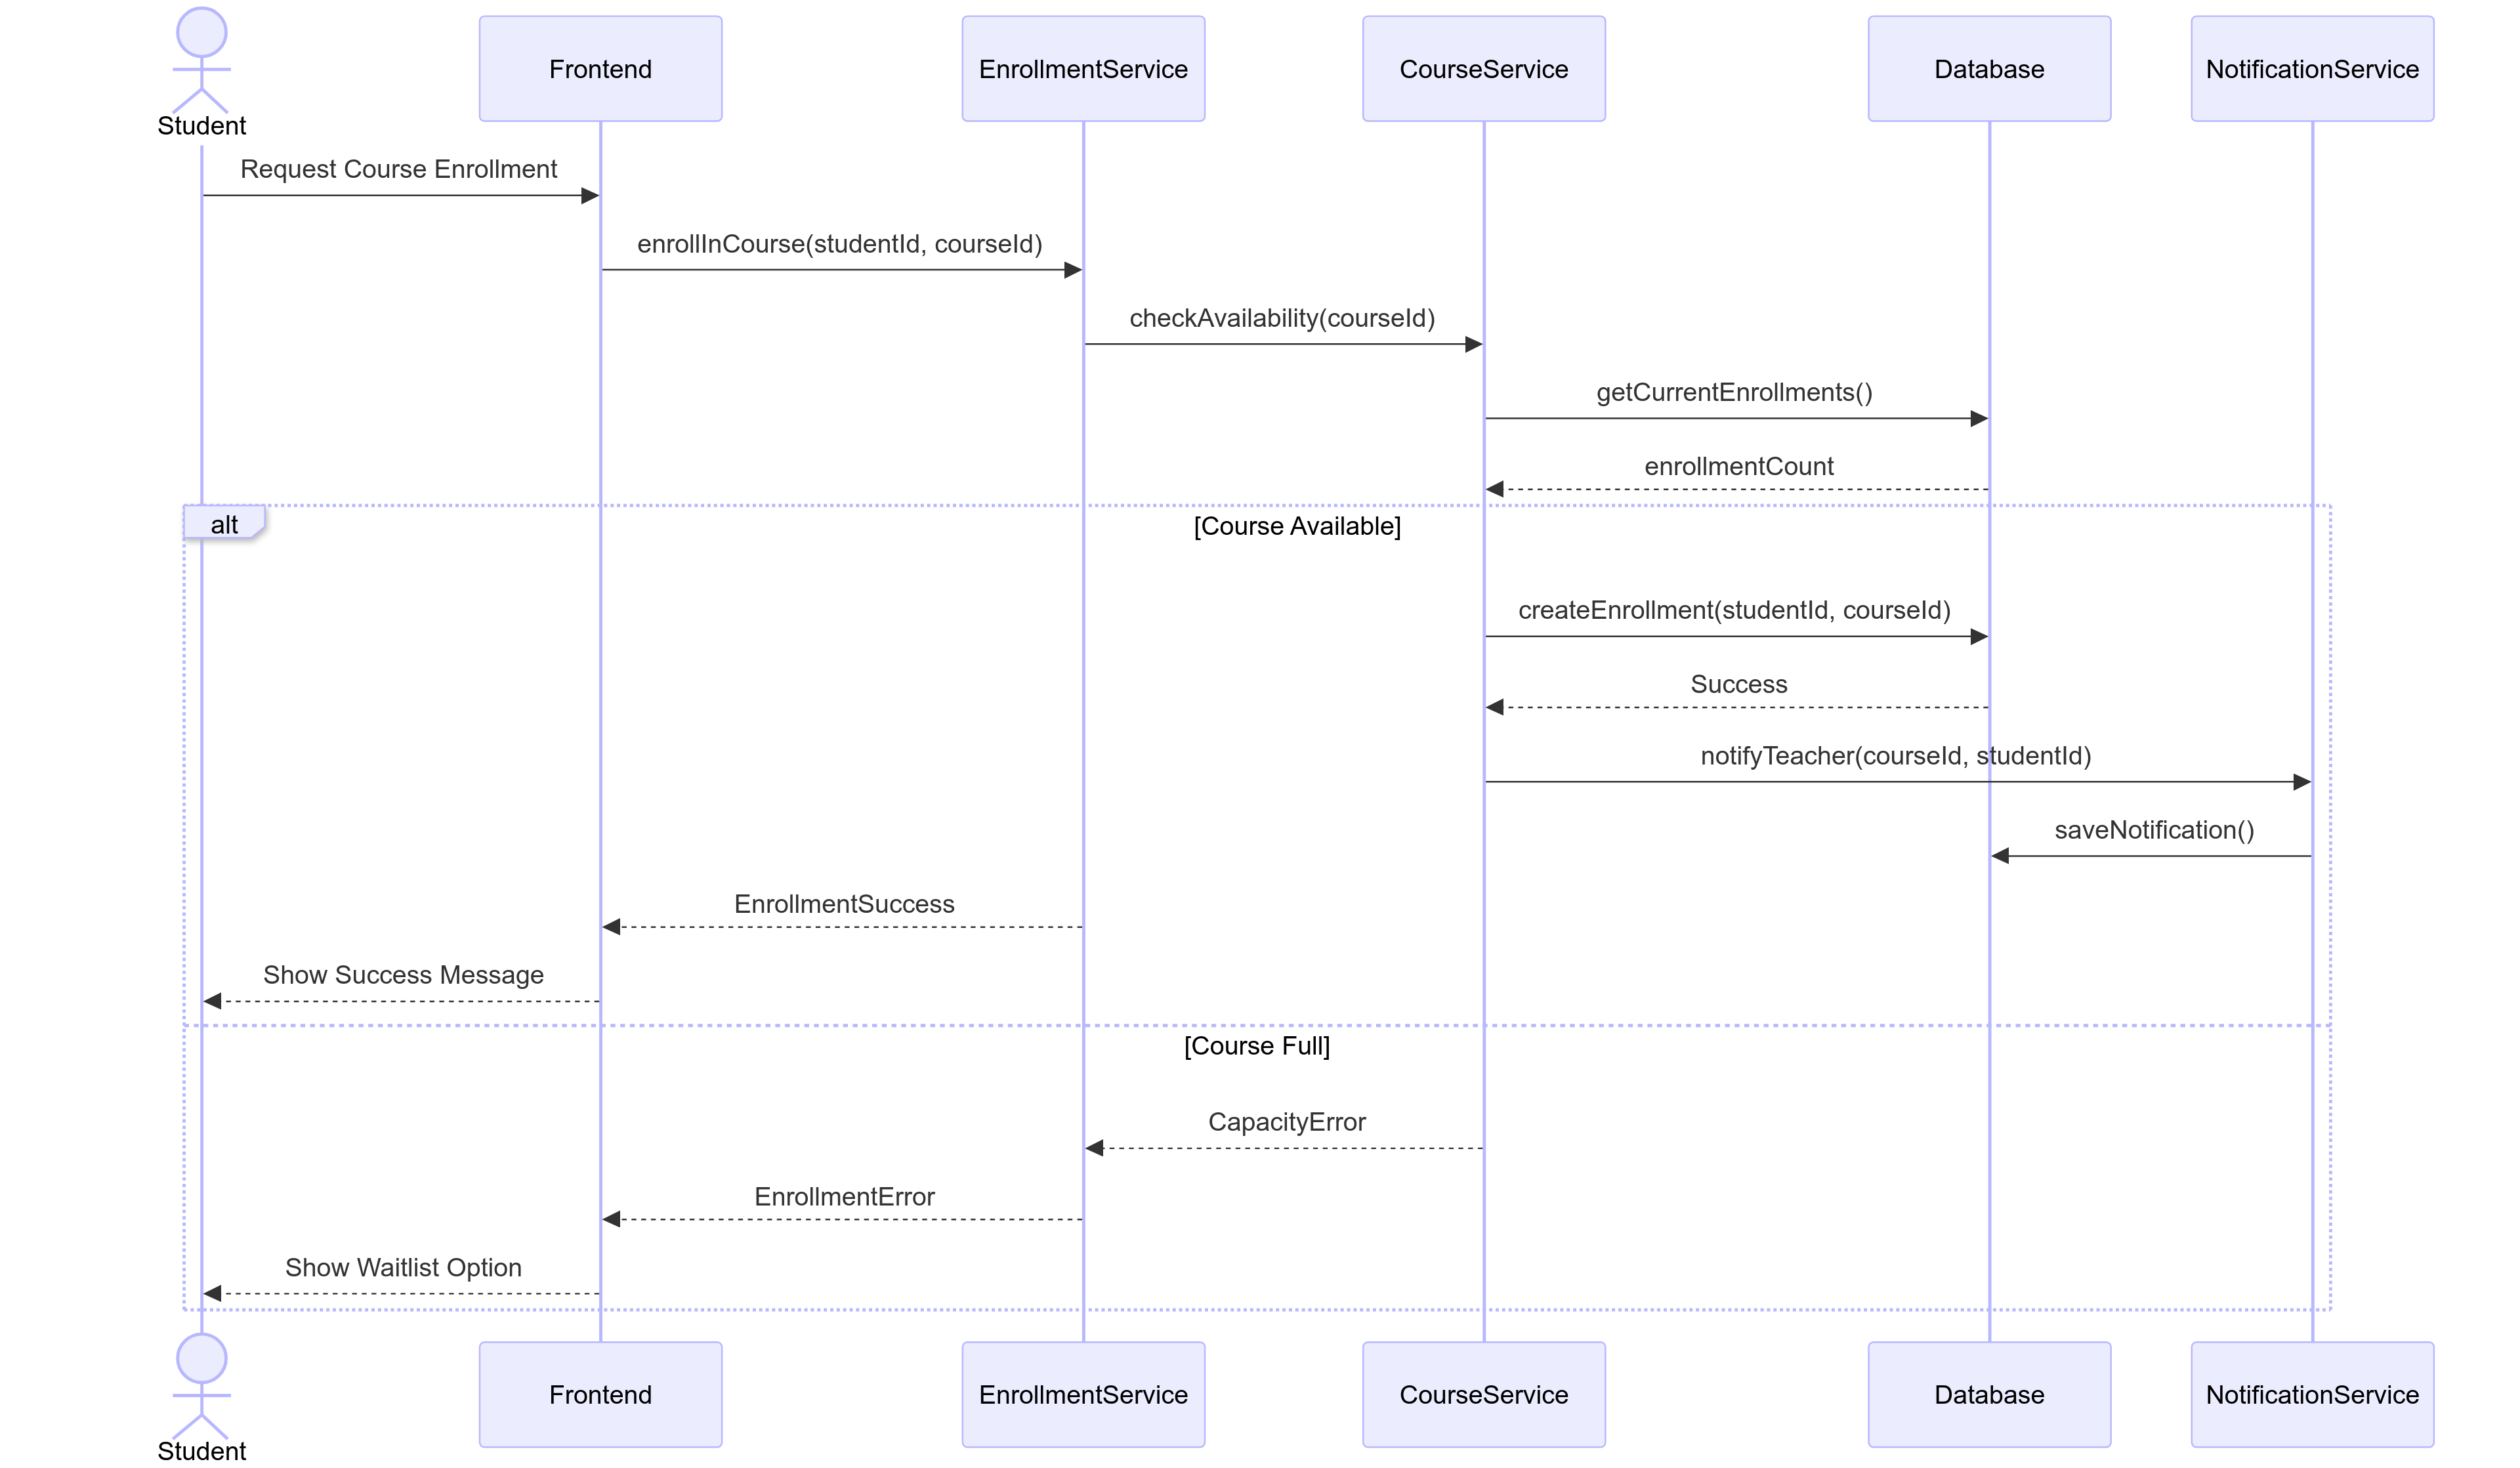
\includegraphics[width=0.9\textwidth,keepaspectratio]{pfe-pics/diagrames/Course Enrollment Process.png}
  \caption{\textbf{Diagramme de flux} pour l'inscription aux cours.}
  \label{fig:course_enrollment}
\end{figure}

Ce diagramme présente :

\begin{itemize}
  \item La recherche et sélection de cours par l'étudiant
  
  \item La vérification des prérequis et disponibilités
  
  \item Le processus d'approbation si nécessaire
  
  \item La confirmation de l'inscription et l'accès au matériel du cours
\end{itemize}

\subsection{Cas d'utilisation}

Le diagramme des cas d'utilisation offre une vue d'ensemble des fonctionnalités du système par type d'utilisateur :

\begin{figure}[H]
  \centering
  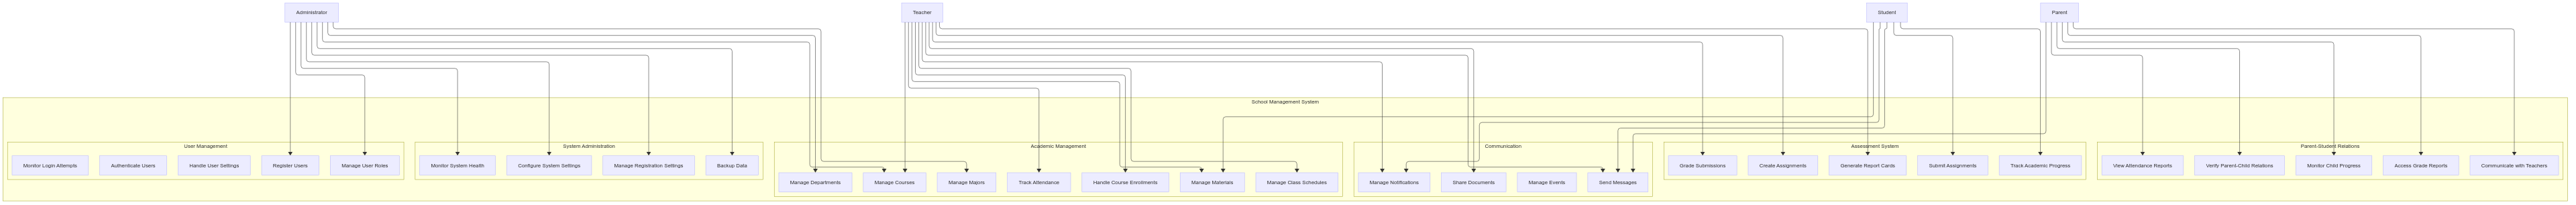
\includegraphics[width=0.9\textwidth,keepaspectratio]{pfe-pics/diagrames/usecase.png}
  \caption{\textbf{Diagramme de cas d'utilisation} du système de gestion scolaire.}
  \label{fig:use_cases}
\end{figure}

Ce diagramme met en évidence :

\begin{itemize}
  \item Les acteurs principaux du système (administrateur, enseignant, étudiant, parent)
  
  \item Les fonctionnalités accessibles à chaque type d'utilisateur
  
  \item Les relations entre les différents cas d'utilisation
  
  \item Les extensions et inclusions entre cas d'utilisation
\end{itemize}

\section{Conception détaillée du système de création de profils IA}

\subsection{Architecture des composants}

L'architecture du système de création de profils IA s'articule autour de plusieurs composants spécialisés :

\begin{figure}[H]
  \centering
  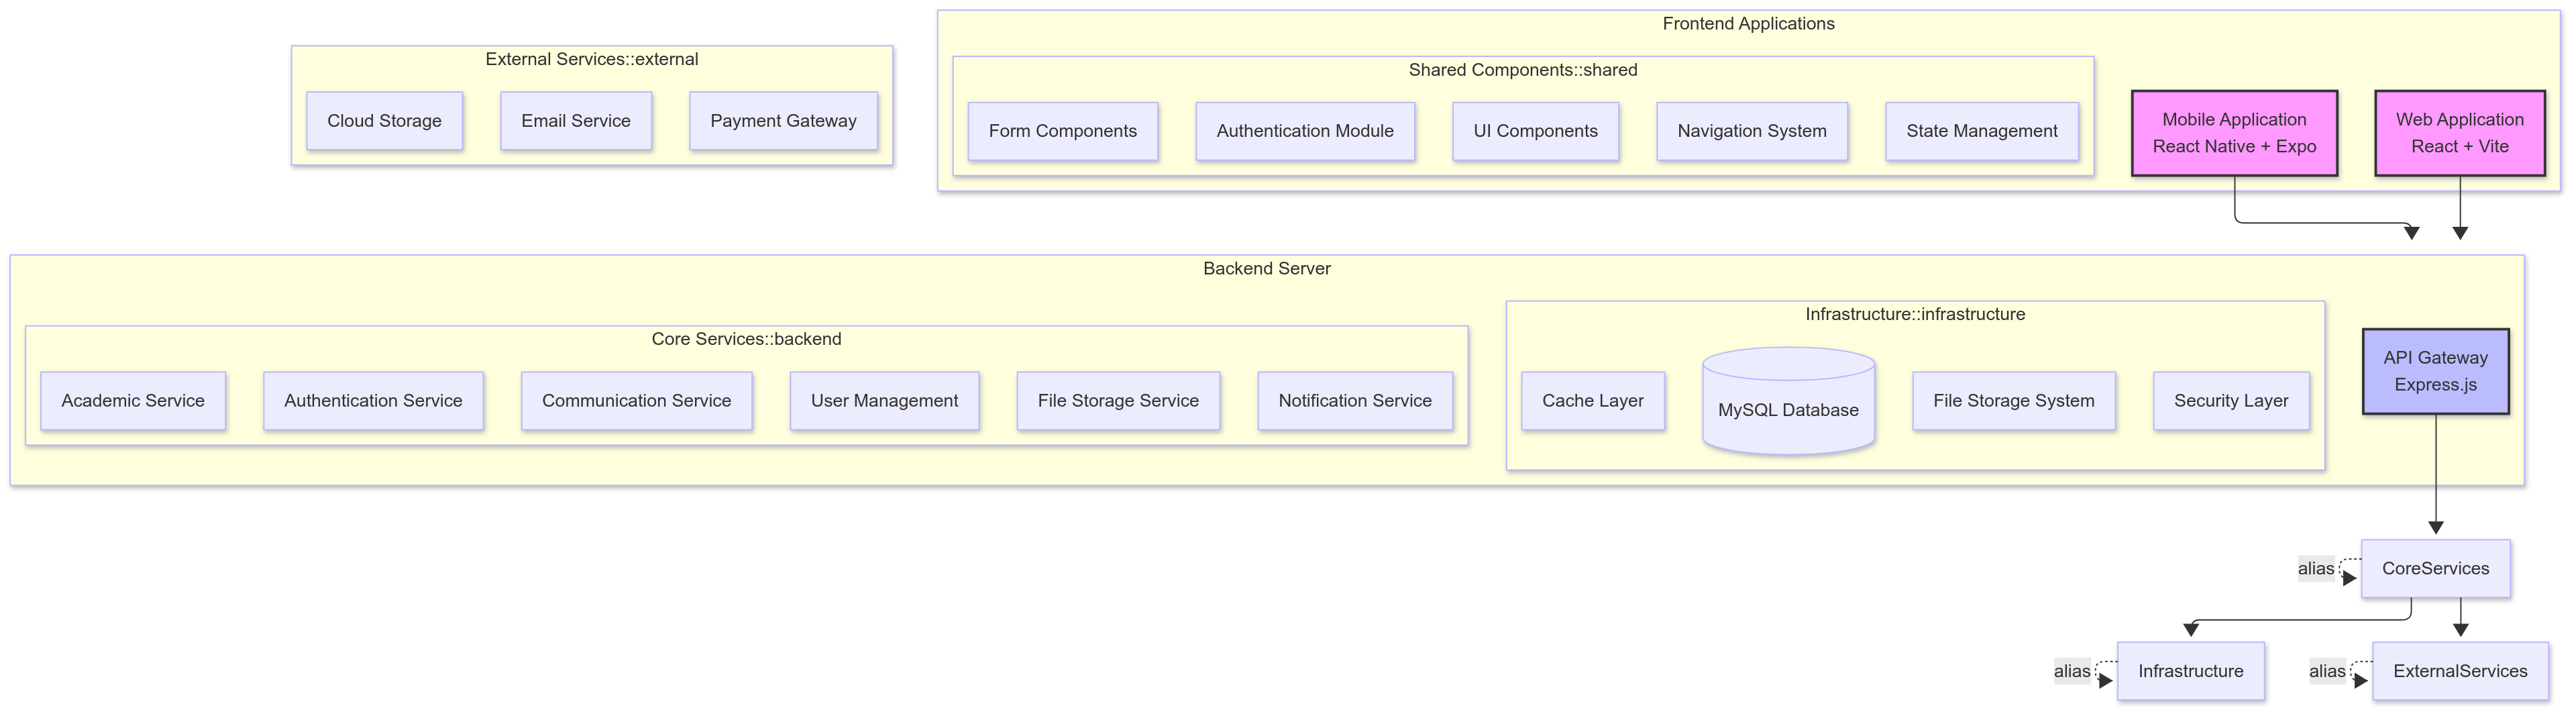
\includegraphics[width=0.9\textwidth,keepaspectratio]{pfe-pics/diagrames/Component Diagram (showing the system_s architecture).png}
  \caption{\textbf{Diagramme de composants} du système de création de profils IA.}
  \label{fig:ai_components}
\end{figure}

Les principaux composants sont :

\begin{itemize}
  \item \textbf{Gestionnaire de profils} : Création et configuration des profils IA
  
  \item \textbf{Processeur de documents} : Traitement et extraction d'informations à partir des documents uploadés
  
  \item \textbf{Moteur d'indexation} : Organisation des connaissances pour une recherche efficace
  
  \item \textbf{Interface conversationnelle} : Gestion des interactions avec les profils IA
  
  \item \textbf{Gestionnaire d'API} : Exposition des fonctionnalités via une API RESTful
  
  \item \textbf{Système d'authentification} : Gestion des utilisateurs et des accès
\end{itemize}

\subsection{Pipeline de traitement des documents}

Le pipeline de traitement des documents constitue un élément central du système de création de profils IA :

\begin{itemize}
  \item \textbf{Étape 1 - Extraction de texte} : Conversion des différents formats de documents en texte brut
  
  \item \textbf{Étape 2 - Analyse structurelle} : Identification des sections, titres, paragraphes et éléments spéciaux
  
  \item \textbf{Étape 3 - Enrichissement sémantique} : Détection des entités, concepts et relations
  
  \item \textbf{Étape 4 - Chunking intelligent} : Segmentation du contenu en unités de connaissance optimales
  
  \item \textbf{Étape 5 - Indexation vectorielle} : Création d'embeddings pour la recherche sémantique
  
  \item \textbf{Étape 6 - Validation et stockage} : Vérification de la qualité et persistance des données traitées
\end{itemize}

\subsection{Modèle de données}

Le modèle de données du système de création de profils IA est conçu pour gérer efficacement les profils, documents et interactions :

\begin{itemize}
  \item \textbf{Profile} : Définition d'un profil IA avec ses paramètres et métadonnées
  
  \item \textbf{Document} : Information sur les documents sources avec leur statut de traitement
  
  \item \textbf{Chunk} : Segments de contenu extraits des documents
  
  \item \textbf{Embedding} : Représentations vectorielles des chunks pour la recherche sémantique
  
  \item \textbf{Conversation} : Sessions de discussion avec un profil IA
  
  \item \textbf{Message} : Échanges individuels au sein d'une conversation
  
  \item \textbf{ApiKey} : Clés d'accès pour l'intégration externe
  
  \item \textbf{User} : Utilisateurs du système avec leurs permissions
\end{itemize}

\subsection{Flux de traitement des requêtes}

Le traitement d'une requête adressée à un profil IA suit un flux optimisé :

\begin{itemize}
  \item \textbf{Réception de la requête} : Validation et prétraitement de la question utilisateur
  
  \item \textbf{Recherche sémantique} : Identification des chunks les plus pertinents dans la base de connaissances
  
  \item \textbf{Construction du contexte} : Assemblage des informations pertinentes avec l'historique de conversation
  
  \item \textbf{Génération de réponse} : Utilisation du modèle d'IA avec le contexte pour produire une réponse
  
  \item \textbf{Post-traitement} : Formatage, vérification et enrichissement de la réponse
  
  \item \textbf{Enregistrement} : Sauvegarde de l'échange pour référence future et amélioration
\end{itemize}

\subsection{Intégration avec les services externes}

Le système s'intègre avec plusieurs services externes pour optimiser ses fonctionnalités :

\begin{itemize}
  \item \textbf{OpenRouter API} : Accès à différents modèles de langage pour la génération de réponses
  
  \item \textbf{Services de stockage objet} : Stockage efficace des documents originaux et traités
  
  \item \textbf{Services d'OCR} : Extraction de texte à partir d'images et documents scannés
  
  \item \textbf{Services d'authentification} : Intégration possible avec des fournisseurs d'identité externes
\end{itemize}

\section{Intégration des deux systèmes}

\subsection{Points d'intégration}

L'intégration entre le système de gestion scolaire et le système de création de profils IA s'effectue à plusieurs niveaux :

\begin{itemize}
  \item \textbf{Authentification unifiée} : Système SSO permettant une navigation fluide entre les deux plateformes
  
  \item \textbf{Association profils-cours} : Possibilité d'associer des profils IA spécifiques à des cours
  
  \item \textbf{Partage de ressources} : Utilisation des documents pédagogiques du système scolaire comme source pour les profils IA
  
  \item \textbf{Intégration UI} : Widgets permettant d'interagir avec les profils IA directement depuis l'interface du système scolaire
\end{itemize}

\subsection{Architecture d'intégration}

L'architecture d'intégration repose sur une approche API-first :

\begin{itemize}
  \item \textbf{API Gateway} : Point d'entrée unifié gérant le routage vers les services appropriés
  
  \item \textbf{Services d'identité partagés} : Gestion centralisée des utilisateurs et autorisations
  
  \item \textbf{Bus d'événements} : Communication asynchrone entre les systèmes pour les mises à jour et notifications
  
  \item \textbf{Cache distribué} : Optimisation des performances pour les données fréquemment accédées
\end{itemize}

\begin{figure}[H]
  \centering
  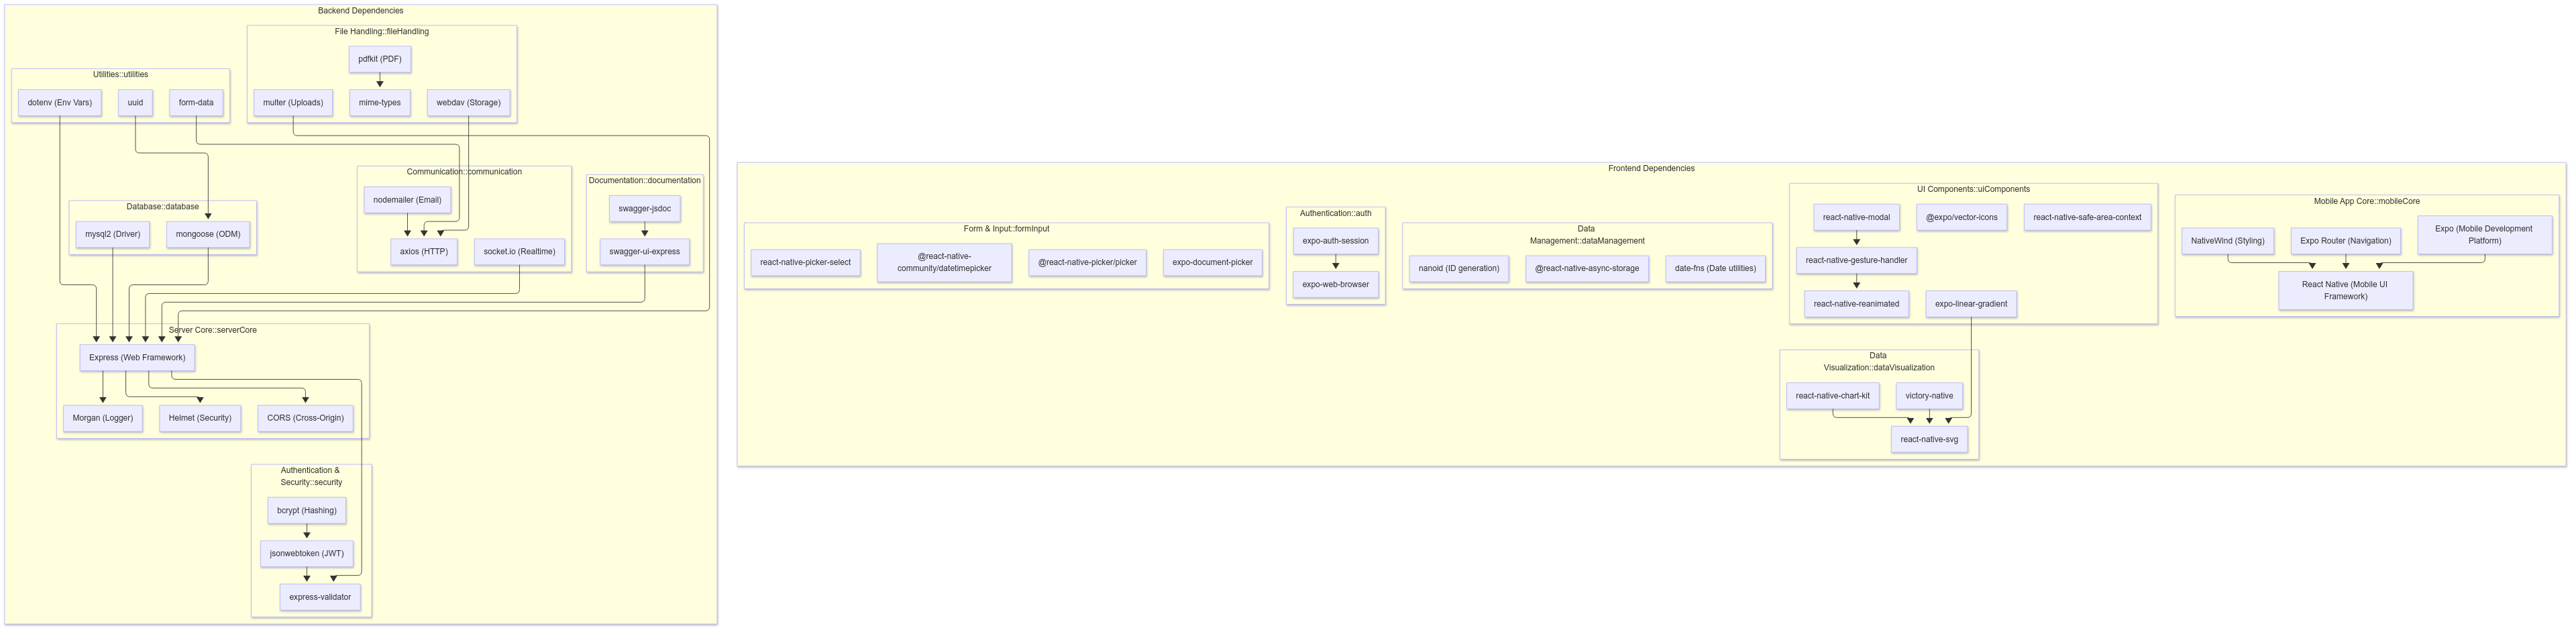
\includegraphics[width=0.9\textwidth,keepaspectratio]{pfe-pics/diagrames/dependeces.png}
  \caption{\textbf{Diagramme de dépendances} montrant l'intégration des systèmes.}
  \label{fig:integration_dependencies}
\end{figure}

\section{Considérations de sécurité et performance}

\subsection{Stratégie de sécurité}

La sécurité a été intégrée à tous les niveaux de la conception :

\begin{itemize}
  \item \textbf{Authentification robuste} : Mécanismes d'authentification modernes avec support MFA
  
  \item \textbf{Autorisation fine} : Contrôle d'accès basé sur les rôles et les ressources
  
  \item \textbf{Protection des données} : Chiffrement des données sensibles au repos et en transit
  
  \item \textbf{Validation des entrées} : Filtrage et validation de toutes les entrées utilisateur
  
  \item \textbf{Audit et journalisation} : Traçabilité des actions sensibles pour détection d'anomalies
  
  \item \textbf{Protection contre les attaques courantes} : Mesures contre XSS, CSRF, injection SQL, etc.
\end{itemize}

\subsection{Optimisation des performances}

Plusieurs stratégies ont été adoptées pour garantir des performances optimales :

\begin{itemize}
  \item \textbf{Mise en cache multicouche} : Cache au niveau du navigateur, de l'API et de la base de données
  
  \item \textbf{Traitement asynchrone} : Utilisation de files d'attente pour les opérations longues
  
  \item \textbf{Pagination et chargement différé} : Optimisation du chargement des données volumineuses
  
  \item \textbf{Optimisation des requêtes} : Indexation et requêtes efficientes sur la base de données
  
  \item \textbf{Distribution de charge} : Répartition du trafic entre plusieurs instances de service
\end{itemize}

\subsection{Stratégie de déploiement}

L'architecture a été conçue pour faciliter un déploiement flexible et évolutif :

\begin{itemize}
  \item \textbf{Conteneurisation} : Packaging des services dans des conteneurs Docker pour portabilité
  
  \item \textbf{Configuration externalisée} : Séparation du code et de la configuration pour adaptation à différents environnements
  
  \item \textbf{Déploiement progressif} : Stratégies de déploiement bleu-vert ou canary pour minimiser les risques
  
  \item \textbf{Surveillance intégrée} : Métriques et alertes pour suivre la santé et les performances du système
\end{itemize}

\section{Gestion de projet}

La réalisation de nos deux systèmes complémentaires a nécessité une planification rigoureuse et une gestion de projet structurée pour garantir l'atteinte des objectifs dans les délais impartis.

\subsection{Approche méthodologique}

Notre approche de gestion de projet s'est appuyée sur une méthodologie hybride combinant :

\begin{itemize}
  \item \textbf{Éléments Agile} : Développement itératif, sessions de revue régulières, adaptation aux retours utilisateurs
  
  \item \textbf{Planification structurée} : Définition claire des jalons et livrables, allocation des ressources
  
  \item \textbf{Gestion des risques} : Identification précoce et stratégies d'atténuation des risques potentiels
\end{itemize}

Cette approche nous a permis de maintenir un équilibre entre la rigueur nécessaire pour un projet académique et la flexibilité requise face aux défis techniques et contraintes temporelles.

\subsection{Organisation temporelle}

Le projet s'est déroulé sur une période de six mois, de novembre 2024 à avril 2025, avec une interruption en fin de période due aux examens nationaux. Le diagramme de Gantt ci-dessous présente la répartition temporelle des différentes phases :

\begin{figure}[H]
  \centering
  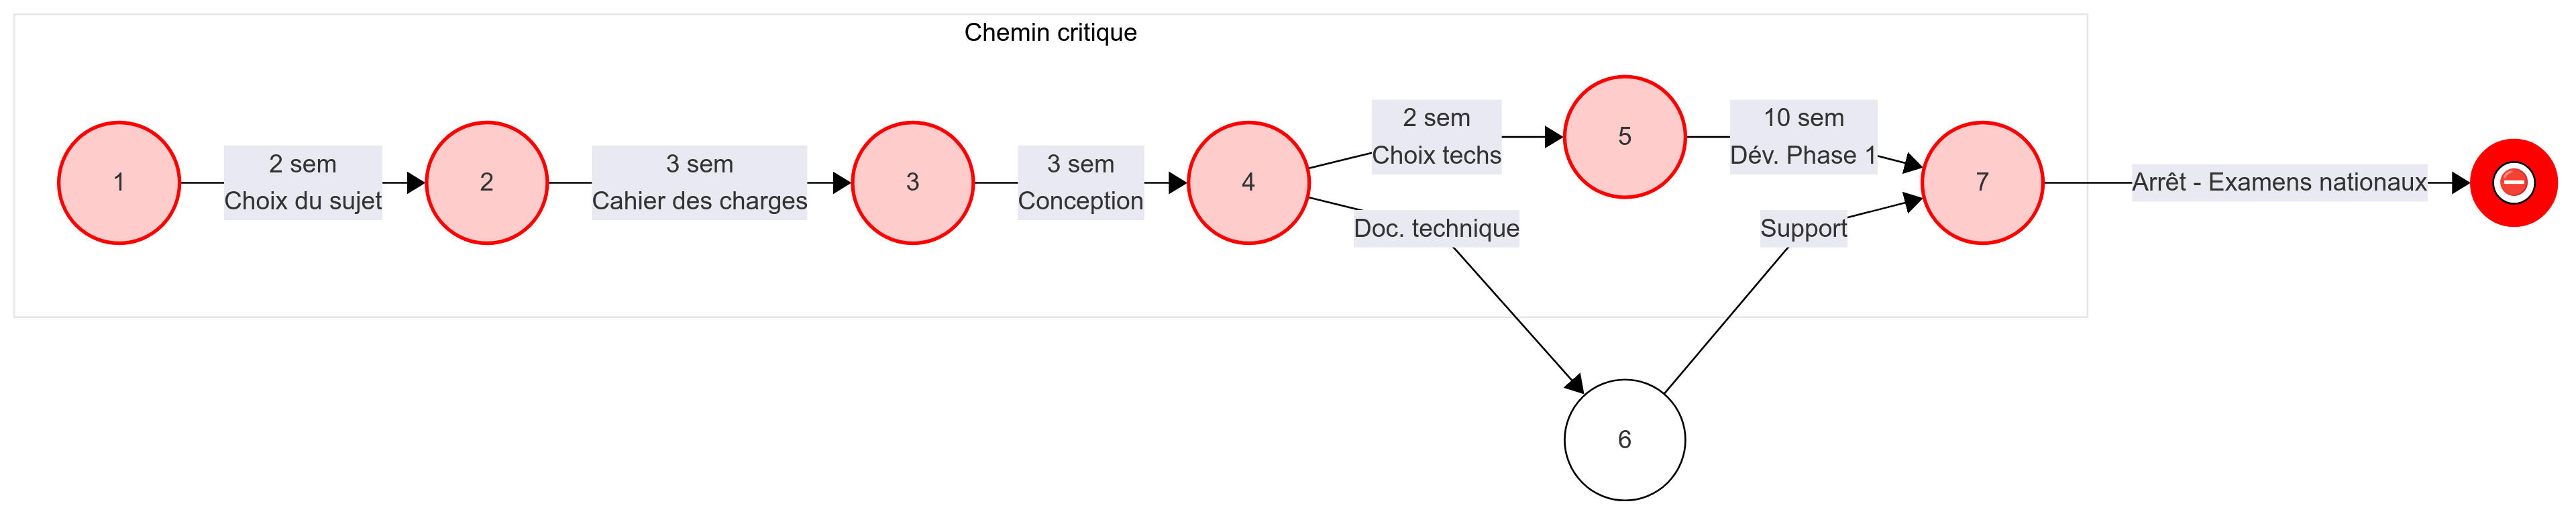
\includegraphics[width=1.0\textwidth,keepaspectratio]{pfe-pics/diagrames/Mermaid Chart - Create complex, visual diagrams with text. A smarter way of creating diagrams.-2025-06-10-203658.png}
  \caption{\textbf{Diagramme de Gantt} montrant la planification temporelle du projet.}
  \label{fig:gantt_chart}
\end{figure}

Les principales phases identifiées sont :

\begin{itemize}
  \item \textbf{Phase d'analyse} (Novembre - Décembre 2024) : Étude des besoins, analyse de l'existant, spécification des exigences
  
  \item \textbf{Phase de conception} (Décembre 2024 - Janvier 2025) : Élaboration des architectures et modèles détaillés
  
  \item \textbf{Phase de développement 1} (Janvier - Février 2025) : Implémentation du système de gestion scolaire
  
  \item \textbf{Phase de développement 2} (Février - Mars 2025) : Implémentation du système de création de profils IA
  
  \item \textbf{Phase d'intégration} (Mars 2025) : Interconnexion des deux systèmes
  
  \item \textbf{Phase de tests et validation} (Mars - début Avril 2025) : Vérification des fonctionnalités et performances
  
  \item \textbf{Phase de documentation} (Avril 2025) : Finalisation de la documentation technique et utilisateur
\end{itemize}

Il est à noter que la phase de développement 2 n'a été que partiellement complétée et que la phase de tests a été limitée en raison des contraintes temporelles liées aux examens nationaux.

\subsection{Dépendances et chemin critique}

Le diagramme PERT ci-dessous illustre les dépendances entre les différentes tâches du projet et met en évidence le chemin critique :

\begin{figure}[H]
  \centering
  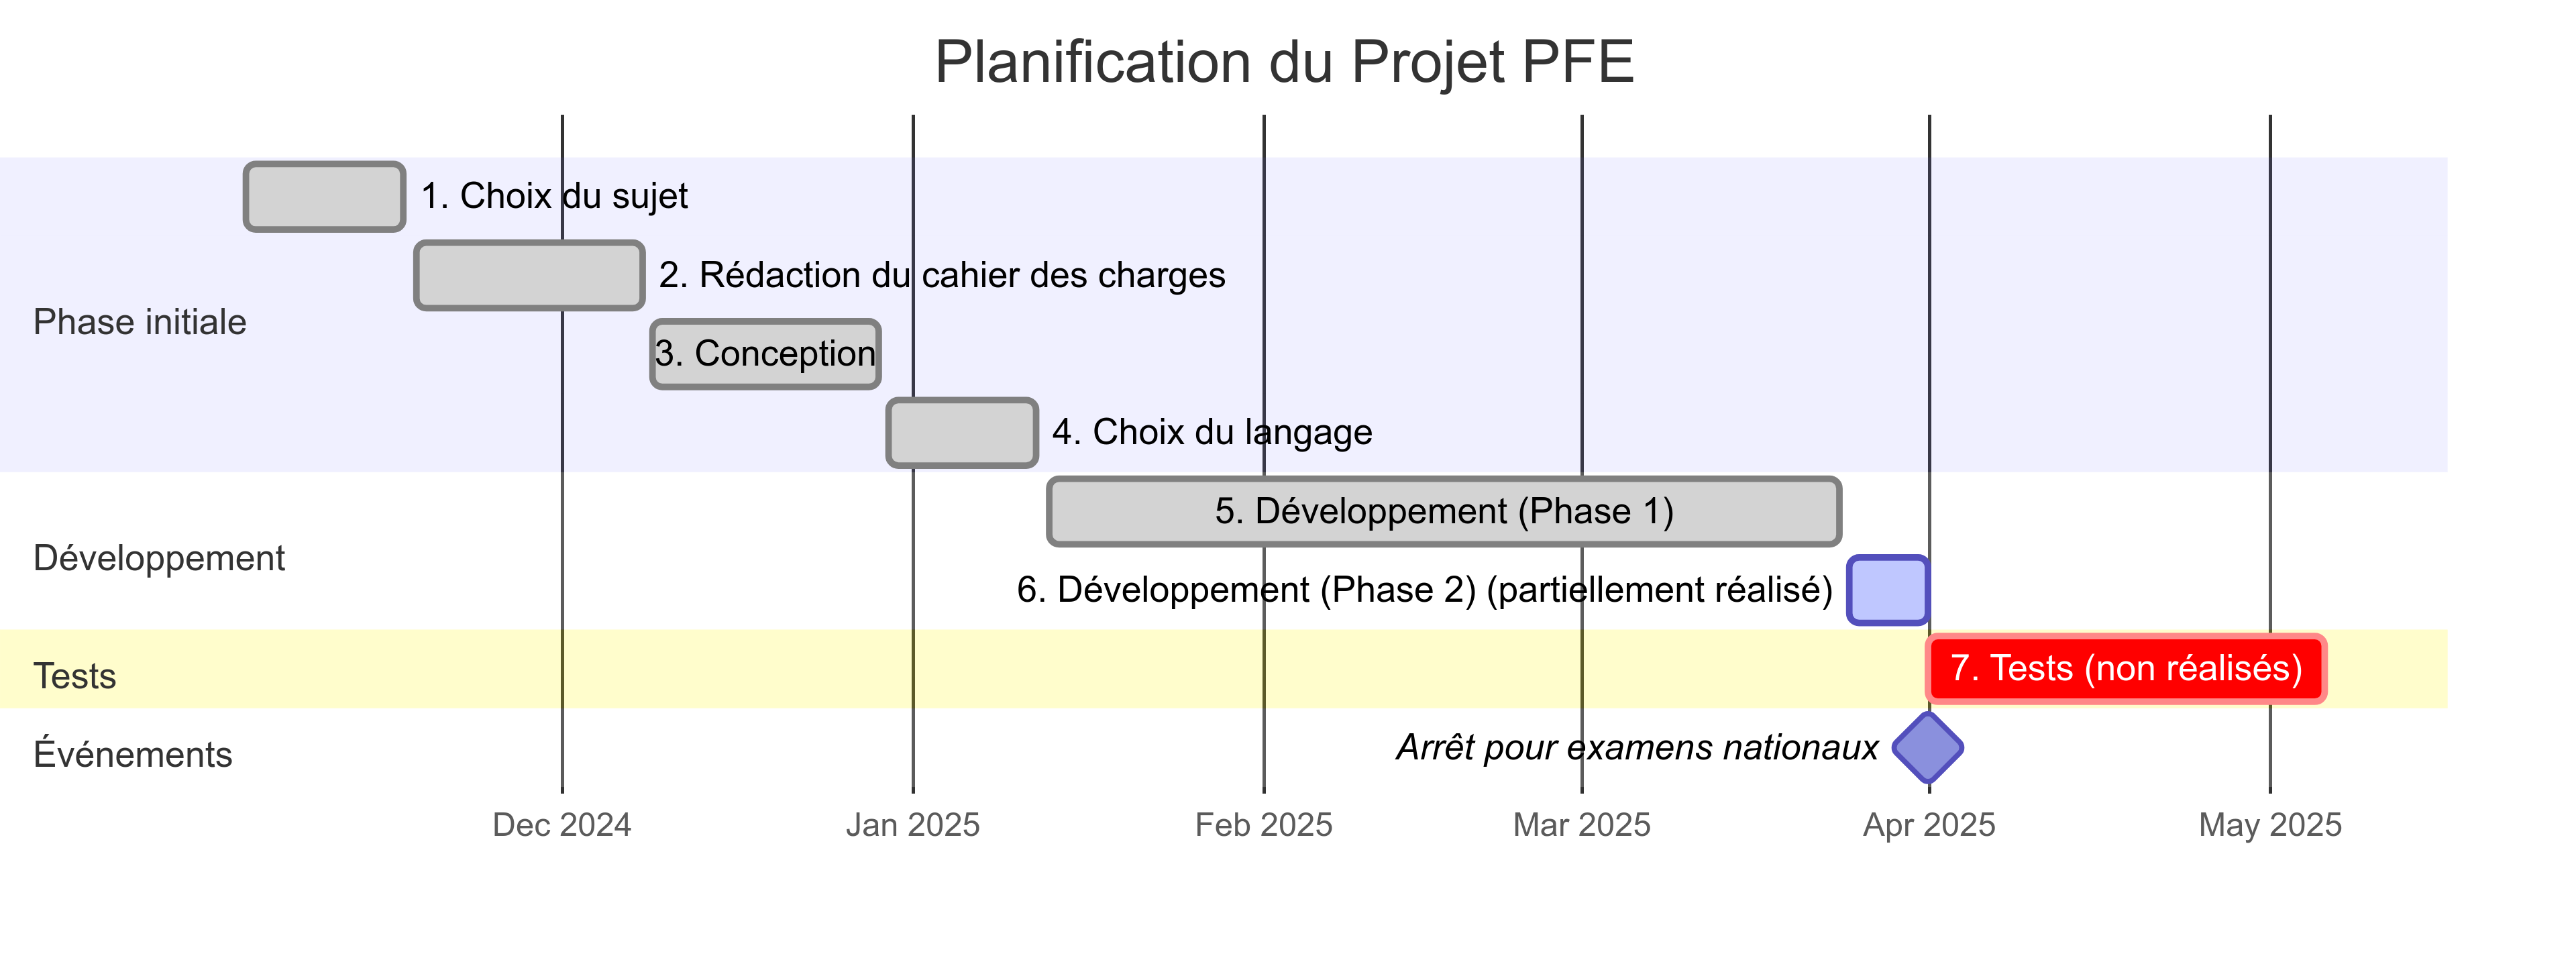
\includegraphics[width=1.0\textwidth,keepaspectratio]{pfe-pics/diagrames/Mermaid Chart - Create complex, visual diagrams with text. A smarter way of creating diagrams.-2025-06-10-203842.png}
  \caption{\textbf{Diagramme PERT} illustrant les dépendances et le chemin critique du projet.}
  \label{fig:pert_diagram}
\end{figure}

Ce diagramme met en évidence :

\begin{itemize}
  \item Les relations de précédence entre les activités
  
  \item Le chemin critique déterminant la durée minimale du projet
  
  \item Les marges disponibles pour certaines activités non critiques
  
  \item Les points de synchronisation nécessaires entre les différents volets du projet
\end{itemize}

L'analyse du chemin critique a révélé que les activités liées à la conception et au développement initial du système de gestion scolaire étaient particulièrement déterminantes pour le respect des délais globaux.

\subsection{Répartition des responsabilités}

Le projet a été mené par une équipe de deux étudiants, avec une répartition des responsabilités basée sur les compétences et centres d'intérêt de chacun :

\begin{itemize}
  \item \textbf{Développement frontend} : Conception et implémentation des interfaces web et mobile
  
  \item \textbf{Développement backend} : Architecture serveur, API et logique métier
  
  \item \textbf{Intégration IA} : Conception et développement du système de création de profils IA
  
  \item \textbf{Base de données} : Modélisation et optimisation des schémas de données
  
  \item \textbf{Tests et validation} : Élaboration et exécution des plans de test
  
  \item \textbf{Documentation} : Rédaction de la documentation technique et utilisateur
\end{itemize}

Cette organisation a permis une progression parallèle sur plusieurs fronts tout en maintenant une cohérence globale grâce à des points de synchronisation réguliers.

\subsection{Gestion des risques}

Une analyse des risques a été réalisée en début de projet, identifiant plusieurs facteurs potentiels d'échec et leurs stratégies d'atténuation :

\begin{itemize}
  \item \textbf{Risque technique} : Complexité de l'intégration IA → Approche progressive avec prototypes
  
  \item \textbf{Risque temporel} : Contraintes liées aux examens → Priorisation des fonctionnalités essentielles
  
  \item \textbf{Risque de coordination} : Communication d'équipe → Outils collaboratifs et réunions régulières
  
  \item \textbf{Risque de périmètre} : Dérive fonctionnelle → Définition claire du MVP et gestion stricte du scope
\end{itemize}

Cette gestion proactive des risques a contribué à maintenir le projet sur les rails malgré plusieurs défis rencontrés en cours de route.

\subsection{Outils de gestion de projet}

Plusieurs outils ont été utilisés pour faciliter la coordination et le suivi du projet :

\begin{itemize}
  \item \textbf{Gestion des tâches} : Trello pour la visualisation des sprints et du backlog
  
  \item \textbf{Gestion du code source} : GitHub avec workflow d'intégration continue
  
  \item \textbf{Communication} : Discord pour les échanges quotidiens et sessions de travail
  
  \item \textbf{Documentation} : Notion pour la documentation évolutive et le partage de ressources
  
  \item \textbf{Suivi du temps} : Toggl pour mesurer l'effort consacré aux différentes tâches
\end{itemize}

Ces outils ont permis de maintenir une visibilité sur l'avancement du projet et de faciliter la collaboration malgré les contraintes de travail à distance.

\section{Conclusion de la conception}

La conception détaillée présentée dans ce chapitre établit une base solide pour l'implémentation de nos deux systèmes complémentaires. L'approche architecturale adoptée privilégie :

\begin{itemize}
  \item La modularité et l'extensibilité pour faciliter l'évolution future
  
  \item La séparation claire des responsabilités pour une maintenance simplifiée
  
  \item L'intégration harmonieuse des deux systèmes pour une expérience utilisateur cohérente
  
  \item La sécurité et la performance comme préoccupations transversales
\end{itemize}

Les diagrammes et modèles élaborés serviront de guide pour la phase d'implémentation, tout en laissant la flexibilité nécessaire pour s'adapter aux défis techniques qui pourraient survenir durant le développement.

L'architecture proposée répond aux exigences fonctionnelles et non fonctionnelles identifiées dans le cahier des charges, et pose les fondations pour des systèmes robustes, évolutifs et centrés sur l'utilisateur. 